\documentclass[pdflatex,sn-mathphys-num]{sn-jnl}% 

\usepackage{graphicx}%
\usepackage{multirow}%
\usepackage{amsmath,amssymb,amsfonts}%
\usepackage{amsthm}%
\usepackage{mathrsfs}%
\usepackage[title]{appendix}%
\usepackage{xcolor}%
\usepackage{textcomp}%
\usepackage{manyfoot}%
\usepackage{booktabs}%
\usepackage{algorithm}%
\usepackage{algorithmicx}%
\usepackage{algpseudocode}%
\usepackage{listings}%
\theoremstyle{thmstyleone}%
\newtheorem{theorem}{Theorem}%  
\newtheorem{proposition}[theorem]{Proposition}% 

\theoremstyle{thmstyletwo}%
\newtheorem{example}{Example}%
\newtheorem{remark}{Remark}%

\theoremstyle{thmstylethree}%
\newtheorem{definition}{Definition}%

\raggedbottom


\begin{document}

\title[Ultra-Lightweight 2D Neural Networks]{Ultra-Lightweight Dense and Recurrent 2D Neural Networks for Edge and Mobile Image Recognition}

\author*[1]{\fnm{Babak} \sur{Shiri}}\email{shiri@njtc.edu.cn}


\author*[2]{\fnm{Zahra} \sur{Alijani}}\email{zahra.alijani@osu.cz}


\affil*[1]{\orgdiv{Key Laboratory of Numerical Simulation of Sichuan Province, School of Mathematics and Big Data}, \orgname{Neijiang Normal University}, \orgaddress{ \city{Neijiang}, \postcode{641100}, \state{Sichuan}, \country{China}}}

\affil*[2]{\orgdiv{Institute for Research and Applications of Fuzzy Modeling, University of Ostrava}, \orgname{University of Ostrava}, \orgaddress{ \city{Ostrava}, \postcode{701 03},  \country{Czech Republic}}}


\abstract{
Ultra-lightweight image recognition is studied using neural networks that keep an image's matrix structure instead of flattening it into a vector, processing it directly through paired left and right linear transformations. Building on this bilinear formulation -- related to prior matrix neural network and matrix-RNN work -- both a dense two-layer architecture and a patch-based recurrent variant are developed and systematically compared across a three-tier parameter budget (super-tiny, tiny, ultra-light). Both variants are evaluated on the MNIST and Fashion-MNIST datasets, reaching competitive classification accuracy with extremely low parameter counts and fast training. A real-time Android application is implemented for handwritten digit recognition, demonstrating practical deployability on resource-constrained edge devices.}



\keywords{2D neural networks, Recurrent neural network, lightweight deep learning, ultra-light networks, MNIST classification, mobile implementation, edge AI.}

%%\pacs[JEL Classification]{D8, H51}

%%\pacs[MSC Classification]{35A01, 65L10, 65L12, 65L20, 65L70}

\maketitle

\section{Introduction}
Traditional deep neural networks often suffer from excessive model size, high computational cost, large memory consumption, and significant energy usage during both training and inference. These drawbacks limit their deployment on resource-constrained devices and raise serious concerns regarding environmental sustainability. This work is motivated by the critical demand for ultra-lightweight neural networks that maintain strong performance while drastically reducing computational overhead. Lighter models enable faster inference, lower memory requirements, reduced energy consumption, and more efficient training.

Various lightweight and efficient learning models have been proposed for visual recognition tasks.
Fundamental techniques for neural network initialization and optimization have been well established in \cite{xavier_glorot, he_init, kingma2014adam}.
Classical frameworks, including support-vector networks \cite{Cortes1995}, backpropagation-based multilayer perceptrons \cite{Rumelhart1986}, and convolutional neural networks \cite{LeCun1998,Krizhevsky2012}, have laid solid foundations for high-precision image classification.
Recently, low-power neuromorphic and optoelectronic neural networks have drawn growing attention for edge computing and mobile applications \cite{Zhu2022, Beyeler2013, Song2024}.
Nevertheless, the performance and efficiency of lightweight architectures that fully preserve the inherent spatial structure of images still can be further improved.
%%%%%%%%%%%

 The growing deployment of artificial intelligence on mobile, IoT, and embedded devices has created a strong demand for lightweight neural networks that achieve high accuracy with limited computational, memory, and energy resources \cite{Han2015, Howard2017, Sandler2018, Tan2019}. Although deep neural networks have achieved remarkable success in image recognition, their complexity often restricts practical deployment on resource-constrained edge platforms. A common limitation of many neural architectures is the vectorization of image inputs before processing. Flattening transforms matrix-valued images into one-dimensional vectors, destroying their inherent spatial organization and weakening the exploitation of structural relationships among pixels \cite{LeCun1998, Kolda2009}. Convolution neural networks partially address this issue through local receptive fields and weight sharing \cite{LeCun1998, Krizhevsky2012}; however, competitive performance typically requires deep architectures with substantial computational cost. To preserve spatial information while reducing model complexity, increasing attention has been directed toward matrix- and tensor-based learning frameworks, which process multidimensional data directly and often achieve favorable parameter efficiency \cite{Kolda2009, Novikov2015, Gao2017MatNet}. From this perspective, bilateral transformations acting simultaneously along row and column dimensions provide a natural mechanism for exploiting two-dimensional image structure. Moreover, recurrent processing can be adapted from temporal sequences to spatial image patches, enabling iterative context aggregation with low computational overhead \cite{Hochreiter1997, Graves2006}. Matrix-valued recurrent formulations have also been studied directly: Renanse et al. \cite{Renanse2023} analyze the memory capacity of RNNs whose hidden state is itself a matrix updated through the same bilinear map $Y=UXV+B$ used here and in MatNet, within a general sequence-memory framework rather than image classification, while Graves et al. \cite{Graves2007MDRNN} introduced Multi-Dimensional RNNs that propagate hidden states across a full two-dimensional grid of local windows, each cell receiving input from multiple spatial predecessors, later applied to texture and scene classification through 2D-LSTM networks \cite{Byeon2014}. The 2D-RNN developed in Section~\ref{2D-RNN} differs from these in scope and mechanism: it propagates hidden state along a single raster-order chain over patches (each hidden state depending on one spatial predecessor rather than a full multi-directional grid), separates a bilinear feature-projection stage from the bilinear recurrent update, and targets ultra-lightweight parameter budgets and mobile deployment rather than general sequence memory or full-scale scene labeling. Motivated by these observations, this work investigates both dense two-dimensional neural networks and recurrent two-dimensional neural networks within a unified matrix-learning framework for lightweight image recognition.
%%%%%%%%%%%%
Beyond computational burdens, conventional linear transformation mechanisms in basic network designs exhibit inherent structural limitations. Given an input image matrix $\boldsymbol{X}$ and learnable weight matrix $\boldsymbol{W}$, the output feature representation $\boldsymbol{Y}$ is given by
\[
\boldsymbol{Y} = \boldsymbol{W}\boldsymbol{X}.
\]
Each entry can be written as
\[
Y_{ij} = \sum_{p} W_{ip} X_{pj}.
\]
This formulation shows that the feature value $Y_{ij}$ at position $(i,j)$ depends only on the $j$-th column of $\boldsymbol{X}$. Elements from other columns and spatial regions provide no contribution. Standard right-multiplication captures correlations only along the row dimension and ignores cross-column spatial dependencies. Such restricted information flow weakens spatial context modeling and limits feature representation capability.


 Recurrent neural networks (RNNs) have undergone substantial development over the past four decades. Early foundations were established by Hopfield \cite{Hopfield1982}, Jordan \cite{Jordan1986}, and Elman \cite{Elman1990}, while Werbos \cite{Werbos1990} introduced the Backpropagation Through Time (BPTT) algorithm for recurrent learning. The difficulty of learning long-term dependencies due to vanishing and exploding gradients was later identified by Bengio \textit{et al.} \cite{Bengio1994}, motivating the development of Long Short-Term Memory (LSTM) networks by Hochreiter and Schmidhuber \cite{Hochreiter1997} and Bidirectional RNNs by Schuster and Paliwal \cite{Schuster1997}. Subsequent advances included the forget gate \cite{Gers2000}, Connectionist Temporal Classification \cite{Graves2006}, RNN language models \cite{Mikolov2010}, gradient stabilization techniques \cite{Pascanu2013}, the Gated Recurrent Unit (GRU) \cite{Cho2014GRU}, sequence-to-sequence learning \cite{Sutskever2014}, and attention mechanisms \cite{Bahdanau2014}. Although Transformer architectures \cite{Vaswani2017} have largely replaced traditional RNNs in many applications, recent studies have renewed interest in efficient recurrent models for long-sequence processing \cite{Feng2024}. Recent research has also incorporated fractional-order dynamics into recurrent architectures. Unlike conventional RNNs with fixed integer-order memory, fractional recurrent neural networks introduce long-range memory effects through fractional operators. Shiri \textit{et al.} \cite{Shiri2026FRNN} proposed Incommensurate Fractional Recurrent Neural Networks (FRNNs), in which different hidden-state components possess distinct learnable fractional orders. Their results demonstrated that fractional memory dynamics can enhance sequential learning while providing a richer mathematical framework for recurrent computation. 
In particular \cite{Shiri2026Math}, the existence-uniqueness and Hyers–Ulam stability of generalized incommensurate fractional differential systems, together with their neural network applications, were rigorously established in \cite{Shiri2026Math}.
At the level of individual neurons, Molek and Alijani \cite{Molek2025PRL} treated fractional-order derivatives as trainable parameters of the activation functions, showing that fractional variants of the sigmoid, GELU and Mish can improve accuracy on standard vision backbones, albeit at a considerable cost in training time and memory — an overhead that is prohibitive in the ultra-lightweight setting considered here.
Motivated by recent advances in matrix-valued learning and recurrent processing, this study investigates two complementary lightweight architectures. The first is a dense two-dimensional neural network that preserves image structure through bilateral matrix transformations without vectorization. The second is a two-dimensional recurrent architecture that processes spatial image patches through recursive hidden-state propagation. Together, these models aim to achieve efficient image recognition with low parameter counts, making them suitable for real-time edge and mobile applications. 
This work also fits into a broader research direction on digital technologies for wellbeing. Here, wellbeing data are often non-numeric: images, handwriting, drawings, and other unstructured records that social scientists usually analyze only with qualitative methods. Lightweight matrix-based networks such as those proposed here can process this kind of data directly and cheaply on personal and edge devices, so sensitive data can stay on the device.

%%%%%%%
To overcome both the high computational cost of deep models and the insufficient spatial modeling of traditional linear operations, this paper studies an ultra-lightweight class of two-dimensional neural networks, building on established bilinear/matrix-network formulations \cite{Gao2017MatNet, Renanse2023}. Experiments are performed using the shallowest possible structure with only two layers. Evaluations are carried out under a well-defined classification of lightweight network scales:
\begin{itemize}
    \item Super Tiny Ultra-Light: less than 1K parameters
    \item Tiny Ultra-Light: 1K--10K parameters
    \item Ultra-Light: 10K--100K parameters
\end{itemize}

The main contributions of this work are summarized as follows:

\begin{itemize}
    \item A dense 2D neural-network layer using paired left-right bilinear transformations is presented, related to prior matrix neural network formulations (e.g., MatNet \cite{Gao2017MatNet}) but instantiated as a minimal two-layer classifier and systematically evaluated at parameter budgets well below prior work.
    \item A three‑tier lightweight taxonomy (super‑tiny, tiny, ultra‑light) is established for standardized model evaluation.
    \item  A shallow two‑layer dense 2D‑NN is demonstrated to yield competitive accuracy on MNIST and Fashion‑MNIST under low‑parameter constraints.
    \item A patch-based 2D-RNN variant, related to prior matrix-RNN and multi-dimensional RNN formulations \cite{Renanse2023, Graves2007MDRNN} but using a simpler single-direction raster-order recurrence, is developed for spatial recurrent learning, and key accuracy‑speed‑parameter trade‑offs are uncovered via systematic ablation experiments.
    \item A real‑time Android application is implemented, through which the deployability of the lightweight models on resource‑constrained edge devices is validated.
    
\end{itemize}


Section \ref{2D Neural Networks} introduces the proposed two-dimensional dense neural network framework and derives its forward propagation and backpropagation algorithms directly in matrix form. The resulting architecture preserves the inherent spatial structure of image data while avoiding vectorization operations. Section \ref{Experimental Results} presents empirical evaluations on the MNIST handwritten digit benchmark, including performance analysis under multiple ultra-lightweight parameter regimes and implementation on mobile devices. Section \ref{2D-RNN} extends the matrix-learning philosophy to a recurrent setting by developing a two-dimensional recurrent neural network (2D-RNN) operating on image patches. Comparative experiments between dense and recurrent architectures are subsequently conducted to investigate the trade-offs among classification accuracy, parameter efficiency, and computational cost. Finally, Section \ref{Experiments and Comparative Analysis} summarizes the main findings and discusses future research directions toward lightweight matrix-based intelligence for edge computing applications.
\section{2D Neural Networks}\label{2D Neural Networks}
Images are naturally represented as two- or three-dimensional numerical arrays. This raises a fundamental research question: why are such inherent 2D spatial structures rarely preserved in standard neural network designs? In most conventional frameworks, matrix-shaped inputs are flattened into one-dimensional vectors before processing. This work investigates whether high-quality feature learning and competitive classification performance can be achieved directly on raw matrix inputs without destructive flattening operations.

To address this question, we consider a generic input matrix $\boldsymbol{X} \in \mathbb{R}^{\mu_1 \times \nu_1}$ with initial size $\mu_1 \times \nu_1$. The core objective of each network layer is to map this input to a new feature matrix $\boldsymbol{Z}^{[1]}$ of target dimension $\mu_2 \times \nu_2$. First, a left-side linear transformation is applied via a learnable weight matrix $\boldsymbol{W}^{[L1]} \in \mathbb{R}^{\mu_2 \times \mu_1}$, producing an intermediate feature matrix of size $\mu_2 \times \nu_1$. To adapt the second spatial dimension, a complementary right-side multiplication is further performed using $\boldsymbol{W}^{[R1]} \in \mathbb{R}^{\nu_1 \times \nu_2}$.

The complete construction of the first network layer is formulated as
\begin{align}
\boldsymbol{Z}^{[L1]}_{\mu_2 \times \nu_1} &= \boldsymbol{W}^{[L1]}_{\mu_2 \times \mu_1} \boldsymbol{X}_{\mu_1 \times \nu_1} + \boldsymbol{B}^{[L1]}_{\mu_2 \times \nu_1}, \\
\boldsymbol{Z}^{[1]}_{\mu_2 \times \nu_2}  &= \boldsymbol{Z}^{[L1]}_{\mu_2 \times \nu_1} \boldsymbol{W}^{[R1]}_{\nu_1 \times \nu_2} + \boldsymbol{B}^{[R1]}_{\mu_2 \times \nu_2},
\end{align}
where $\boldsymbol{B}^{[L1]}$ and $\boldsymbol{B}^{[R1]}$ denote learnable bias matrices. Substituting the first equation into the second yields a compact combined expression:
\[
\boldsymbol{Z}^{[1]}
=
\boldsymbol{W}^{[L1]} \boldsymbol{X} \boldsymbol{W}^{[R1]}
+ \boldsymbol{B}^{[L1]} \boldsymbol{W}^{[R1]}
+ \boldsymbol{B}^{[R1]}.
\]
Since the term $\boldsymbol{B}^{[L1]} \boldsymbol{W}^{[R1]}$ is input-independent and constant during forward propagation, it can be merged into a single unified bias term $\boldsymbol{B}^{[1]}$. Accordingly, the pre-activation output of the 2D layer simplifies to
\begin{equation}
\boldsymbol{Z}^{[1]}_{\mu_2 \times \nu_2}
=
\boldsymbol{W}^{[L1]}_{\mu_2 \times \mu_1}
\boldsymbol{X}_{\mu_1 \times \nu_1}
\boldsymbol{W}^{[R1]}_{\nu_1 \times \nu_2}
+ \boldsymbol{B}^{[1]}_{\mu_2 \times \nu_2}.
\end{equation}

Subsequently, a nonlinear activation function
\[
F^{[1]}: \mathbb{R}^{\mu_2 \times \nu_2} \to \mathbb{R}^{\mu_2 \times \nu_2}
\]
is applied element-wise to introduce nonlinearity, producing the final first-layer output:
\begin{equation}
\boldsymbol{Y}^{[1]}_{\mu_2 \times \nu_2}
=
F^{[1]}\bigl(\boldsymbol{Z}^{[1]}_{\mu_2 \times \nu_2}\bigr).
\end{equation}

By extension, a deep 2D neural network with total depth $d$ can be defined through recursive layer-wise propagation:
\begin{equation}
\begin{split}
\boldsymbol{Z}^{[1]}_{\mu_2 \times \nu_2}
&=
\boldsymbol{W}^{[L1]}_{\mu_2 \times \mu_1}
\boldsymbol{X}_{\mu_1 \times \nu_1}
\boldsymbol{W}^{[R1]}_{\nu_1 \times \nu_2}
+ \boldsymbol{B}^{[1]}_{\mu_2 \times \nu_2},\\
\boldsymbol{Y}^{[1]}_{\mu_2 \times \nu_2}
&=
F^{[1]}\bigl(\boldsymbol{Z}^{[1]}_{\mu_2 \times \nu_2}\bigr),\\
\boldsymbol{Z}^{[2]}_{\mu_3 \times \nu_3}
&=
\boldsymbol{W}^{[L2]}_{\mu_3 \times \mu_2}
\boldsymbol{Y}^{[1]}_{\mu_2 \times \nu_2}
\boldsymbol{W}^{[R2]}_{\nu_2 \times \nu_3}
+ \boldsymbol{B}^{[2]}_{\mu_3 \times \nu_3},\\
\boldsymbol{Y}^{[2]}_{\mu_3 \times \nu_3}
&=
F^{[2]}\bigl(\boldsymbol{Z}^{[2]}_{\mu_3 \times \nu_3}\bigr),\\
&\ \vdots\\
\boldsymbol{Z}^{[d]}_{\mu_{d+1} \times \nu_{d+1}}
&=
\boldsymbol{W}^{[Ld]}_{\mu_{d+1} \times \mu_d}
\boldsymbol{Y}^{[d-1]}_{\mu_d \times \nu_d}
\boldsymbol{W}^{[Rd]}_{\nu_d \times \nu_{d+1}}
+ \boldsymbol{B}^{[d]}_{\mu_{d+1} \times \nu_{d+1}},\\
\boldsymbol{Y}^{[d]}_{\mu_{d+1} \times \nu_{d+1}}
&=
F^{[d]}\bigl(\boldsymbol{Z}^{[d]}_{\mu_{d+1} \times \nu_{d+1}}\bigr).
\end{split}
\end{equation}

Let $\boldsymbol{X}_i$ denote the matrix-form training samples and $\boldsymbol{O}_i$ denote the corresponding target outputs for $i\in I_T$, where $I_T$ represents the index set of the entire training dataset. Network training is formulated as an optimization problem that minimizes the empirical loss function $L(\boldsymbol{Y}^{[d]}_i,\boldsymbol{O}_i)$.

Denote the gradient of the loss with respect to the final-layer output as $\nabla_{\boldsymbol{Y}^{[d]}_i} L$. The gradient with respect to the pre-activation matrix is computed as
\begin{equation}
\nabla_{\boldsymbol{Z}^{[d]}_i} L
=
\nabla_{\boldsymbol{Y}^{[d]}_i} L
\circ
D_\circ\! F^{[d]}\bigl(\boldsymbol{Z}_i^{[d]}\bigr),
\end{equation}
in which $\circ$ indicates the Hadamard (element-wise) product, and $D_\circ$ denotes the element-wise differentiation of the activation function.

Backpropagation is derived to compute gradients for all learnable parameters. For the output layer $\ell=d$, the gradient formulas are given by
\begin{align*}
\nabla_{\boldsymbol{W}^{[Ld]}} L
&=
\sum_{i\in I_T}
\nabla_{\boldsymbol{Z}_i^{[d]}} L
\big(\boldsymbol{W}^{[Rd]}\big)^\top
\left(\boldsymbol{Y}_i^{[d-1]}\right)^\top,
\\
\nabla_{\boldsymbol{W}^{[Rd]}} L
&=
\sum_{i\in I_T}\big(\boldsymbol{Y}_i^{[d-1]}\big)^\top
\big(\boldsymbol{W}^{[Ld]}\big)^\top
\nabla_{\boldsymbol{Z}_i^{[d]}} L,
\\
\nabla_{\boldsymbol{B}^{[d]}} L
&=
\sum_{i\in I_T} \nabla_{\boldsymbol{Z}_i^{[d]}} L,
\\
\nabla_{\boldsymbol{Y}_i^{[d-1]}} L
&=
\big(\boldsymbol{W}^{[Ld]}\big)^\top
\nabla_{\boldsymbol{Z}_i^{[d]}} L
\big(\boldsymbol{W}^{[Rd]}\big)^\top.
\end{align*}

For any general hidden layer $\ell \in \{1,\dots,d-1\}$, we first define
\[
\nabla_{\boldsymbol{Z}_i^{[\ell]}} L
=
\nabla_{\boldsymbol{Y}_i^{[\ell]}} L
\circ
D_\circ F^{[\ell]}\big(\boldsymbol{Z}_i^{[\ell]}\big).
\]
The corresponding gradient rules take the form
\begin{align*}
\nabla_{\boldsymbol{W}^{[L\ell]}} L
&=
\sum_{i\in I_T}
\nabla_{\boldsymbol{Z}_i^{[\ell]}} L
\big(\boldsymbol{W}^{[R\ell]}\big)^\top
(\boldsymbol{Y}_i^{[\ell-1]})^\top,
\\
\nabla_{\boldsymbol{W}^{[R\ell]}} L
&=
\sum_{i\in I_T}\big(\boldsymbol{Y}_i^{[\ell-1]}\big)^\top
\big(\boldsymbol{W}^{[L\ell]}\big)^\top
\nabla_{\boldsymbol{Z}_i^{[\ell]}} L,
\\
\nabla_{\boldsymbol{B}^{[\ell]}} L
&=
\sum_{i\in I_T} \nabla_{\boldsymbol{Z}_i^{[\ell]}} L,
\\
\nabla_{\boldsymbol{Y}_i^{[\ell-1]}} L
&=
\big(\boldsymbol{W}^{[L\ell]}\big)^\top
\nabla_{\boldsymbol{Z}_i^{[\ell]}} L
\big(\boldsymbol{W}^{[R\ell]}\big)^\top.
\end{align*}

For the input boundary case, we set $\boldsymbol{Y}_i^{[0]} = \boldsymbol{X}_i$. The gradient with respect to the input matrix is then
\[
\nabla_{\boldsymbol{X}_i} L
=
\big(\boldsymbol{W}^{[L1]}\big)^\top
\nabla_{\boldsymbol{Z}_i^{[1]}} L
\big(\boldsymbol{W}^{[R1]}\big)^\top.
\]



\section{Experimental Results on MNIST Digit Recognition}\label{Experimental Results}
In this section, $\boldsymbol{X}$ denotes a single sample from the MNIST dataset with standard dimension $\mathbb{R}^{28 \times 28}$.
We employ the shallowest feasible structure of the proposed 2D neural network, consisting of only two layers.

\begin{example}
The complete two-layer architecture is defined as follows:
\begin{description}
\item[Layer 1] $Y^{[1]}: \mathbb{R}^{28\times 28} \to \mathbb{R}^{\mu_2\times \mu_2}$, where $\nu_2 = \mu_2$, with the ReLU activation function.
\item[Layer 2] $\boldsymbol{a}: \mathbb{R}^{\mu_2\times \mu_2} \to \mathbb{R}^{10\times 1}$, with the softmax activation function for final classification.
\end{description}

A customized categorical cross-entropy loss is adopted for MNIST digit recognition:
\begin{equation}\label{CusCatLoss}
\mathcal{L}(\boldsymbol{y}, \boldsymbol{a})
=
\sum_{k=1}^{10}
\biggl[
y_k \max\bigl(0,\, m^{+} - a_k\bigr)^2
+ \gamma\,(1-y_k) \max\bigl(0,\, a_k - m^{-}\bigr)^2
\biggr],
\end{equation}
where $a_k$ denotes the network output for class $k$, and $y_k$ is the corresponding ground-truth label.
The hyperparameters are set as $\gamma=1$, $m^{+}=0.9$, and $m^{-}=0.1$.
The total number of neurons (Num. Neuron) of the proposed 2D-NN-2L is computed by
\[
2(28\mu_2)+\mu_2^2+10\mu_2+\mu_2+10
= \mu_2^2 + 67\mu_2 + 10.
\]

Performance is evaluated under three lightweight scales:
\begin{itemize}
    \item \textbf{Table \ref{tab:1}}: Super Tiny Ultra-Light ($\mu_2 = 1,2,\dots,12$)
    \item \textbf{Table \ref{tab:2}}: Tiny Ultra-Light ($\mu_2 = 13,14,\dots,71$)
    \item \textbf{Table \ref{tab:3}}: Ultra-Light ($\mu_2 = 72,73,\dots,284$)
\end{itemize}
\end{example}

Experimental results for the Super Tiny Ultra-Light models are summarized in Table~\ref{tab:1}.
The performance is compared with several lightweight methods:
\begin{description}
\item[Optoelectronic NN \cite{Zhu2022}] (1024 photonic synapses) Test Accuracy = 94.1\%
\item[Spiking NN \cite{Beyeler2013}] (3136 synapses) Test Accuracy = 92\%
\item[Multilayer incoherent Optoelectronic NN \cite{Song2024}] Test Accuracy = 92.3\% (3 layers)
\end{description}

Results for the Tiny Ultra-Light category are presented in Table~\ref{tab:2}.
All models are trained for 100 epochs.
Better performance can be achieved by increasing the number of epochs;
for instance, the model with $\mu_2=41$ reaches 97.23\% test accuracy after 1000 epochs.
The Tiny Ultra-Light models (under 10K parameters) are compared with classical approaches:
\begin{description}
\item[LeNet-5 \cite{LeCun1998}] (classical CNN, $\approx$ 60K parameters) Test Accuracy = 99.05\%
\item[Support-Vector Networks \cite{Cortes1995}] (RBF kernel) Test Accuracy = 98.6\%
\item[Shallow MLP \cite{Rumelhart1986}] ($\approx$ 10K parameters) Test Accuracy = 97.3\%
\item[Deep CNN \cite{Krizhevsky2012}] (3 conv layers + batch norm) Test Accuracy = 99.4\%
\end{description}

Training is performed using the Adam optimizer, which combines momentum and RMSprop for adaptive learning rate scheduling.
The initial learning rate is set as
\[\eta=\bar{\mathcal{L}}/3,\]
where $\bar{\mathcal{L}}$ denotes the average loss over the training set.
All parameters are initialized with the Xavier scheme for stable convergence.

\begin{table}[htbp]
\centering
\caption{Training parameters and performance for Super Tiny Ultra-Light 2D-NN-2L.
Batch size = 1000, 60 batches, 100 epochs.
$T$: training time per epoch (seconds) on a standard PC.}
\label{tab:1}
\begin{tabular}{|c|c|c|c|c|c|}
\hline
$\nu_2$ & Num. Neuron & Loss   & Train acc & Test acc & $T$ (s) \\
\hline
1    & 78    & 0.5162  & 35.13  & 36.06  & 0.7 \\
2    & 148   & 0.3268  & 68.71  & 70.25  & 0.7 \\
3    & 220   & 0.2512  & 77.52  & 78.61  & 0.8 \\
4    & 294   & 0.1964  & 82.88  & 81.96  & 0.8 \\
5    & 370   & 0.1489  & 86.31  & 87.17  & 0.9 \\
6    & 448   & 0.1236  & 88.79  & 89.39  & 0.9 \\
7    & 528   & 0.1172  & 89.24  & 88.85  & 0.9 \\
8    & 610   & 0.0804  & 92.74  & 92.67  & 1.0 \\
9    & 694   & 0.0698  & 93.75  & 93.77  & 1.0 \\
10   & 780   & 0.0723  & 93.35  & 93.14  & 1.0 \\
11   & 868   & 0.0657  & 93.93  & 94.13  & 1.1 \\
12   & 958   & 0.0514  & 95.35  & 94.78  & 1.1 \\
\hline
\end{tabular}%
\end{table}

\begin{table}[htbp]
\centering
\caption{Training parameters and performance for Tiny Ultra-Light 2D-NN-2L.
Batch size = 1000, 60 batches, 100 epochs (last row: 1000 epochs).}
\label{tab:2}
\begin{tabular}{cccccc}
\toprule
$\nu_2$ & Num. Neuron & Loss    & Train acc & Test acc & $T$ (s) \\
\midrule
13      & 1050  & 0.05451 & 95.16  & 94.58  & 1.2 \\
17      & 1438  & 0.03735 & 96.76  & 95.70  & 1.4 \\
19      & 1644  & 0.03232 & 97.25  & 96.06  & 1.5 \\
23      & 2080  & 0.03264 & 97.15  & 96.10  & 1.6 \\
31      & 3048  & 0.01875 & 98.50  & 96.48  & 2.0 \\
41      & 4438  & 0.01451 & 98.85  & 96.76  & 3.4 \\
47      & 5368  & 0.01065 & 99.27  & 97.15  & 4.6 \\
53      & 6370  & 0.01174 & 99.10  & 97.26  & 5.5 \\
59      & 7444  & 0.00732 & 99.52  & 97.21  & 7.6 \\
67      & 8988  & 0.00609 & 99.59  & 97.47  & 8.9 \\
71      & 9808  & 0.00748 & 99.46  & 97.48  & 9.8 \\
$71^{*}$ & 9808& 0.00289 & 99.79  & 97.53  & 9.8 \\
\bottomrule
\end{tabular}%
%\vspace{0.3cm}
\parbox[t]{\textwidth}{\small{$^{*}$Trained with 1000 epochs.}}
\end{table}

\begin{table}[htbp]
\centering
\caption{Training parameters and performance for Ultra-Light 2D-NN-2L.
Batch size = 1000, 60 batches. Trained with 350 epochs.}
\label{tab:3}
\begin{tabular}{|c|c|c|c|c|c|}
\hline
$\nu_2$ & Num. Neuron & Loss    & Train acc & Test acc & $T$ (s) \\
\hline
284 & 99694& 0.001251  &   99.91       & 98.35
& 150 \\
\hline
\end{tabular}
\end{table}
\subsection{Implementation on Mobile Devices}
We developed an Android application in Kotlin with Jetpack Compose for handwritten digit recognition. The application captures user input via a drawing canvas, converts the handwritten sketch into a normalized 28×28 binary matrix, and performs real-time classification using the proposed lightweight 2D neural network with pre-trained weights (Figure \ref{fig1}). The system also visualizes the digit matrix as a heatmap and supports real-time image preprocessing and inference. The network was trained on the MNIST dataset using rounding operations to generate binary representations.

Experimental evaluation shows minor limitations with highly translated or rotated handwritten digits, leading to a test accuracy of approximately $98.35\%$. It is worth noting that the current implementation does not use feature extraction, patch-based processing, or attention mechanisms. Since training the ultra-lightweight network on a standard CPU takes less than 15 minutes, the proposed method exhibits strong potential for efficient edge AI deployment and further optimization.

\begin{figure}[htbp]
    \centering
    \begin{minipage}{0.32\textwidth}
        \centering
        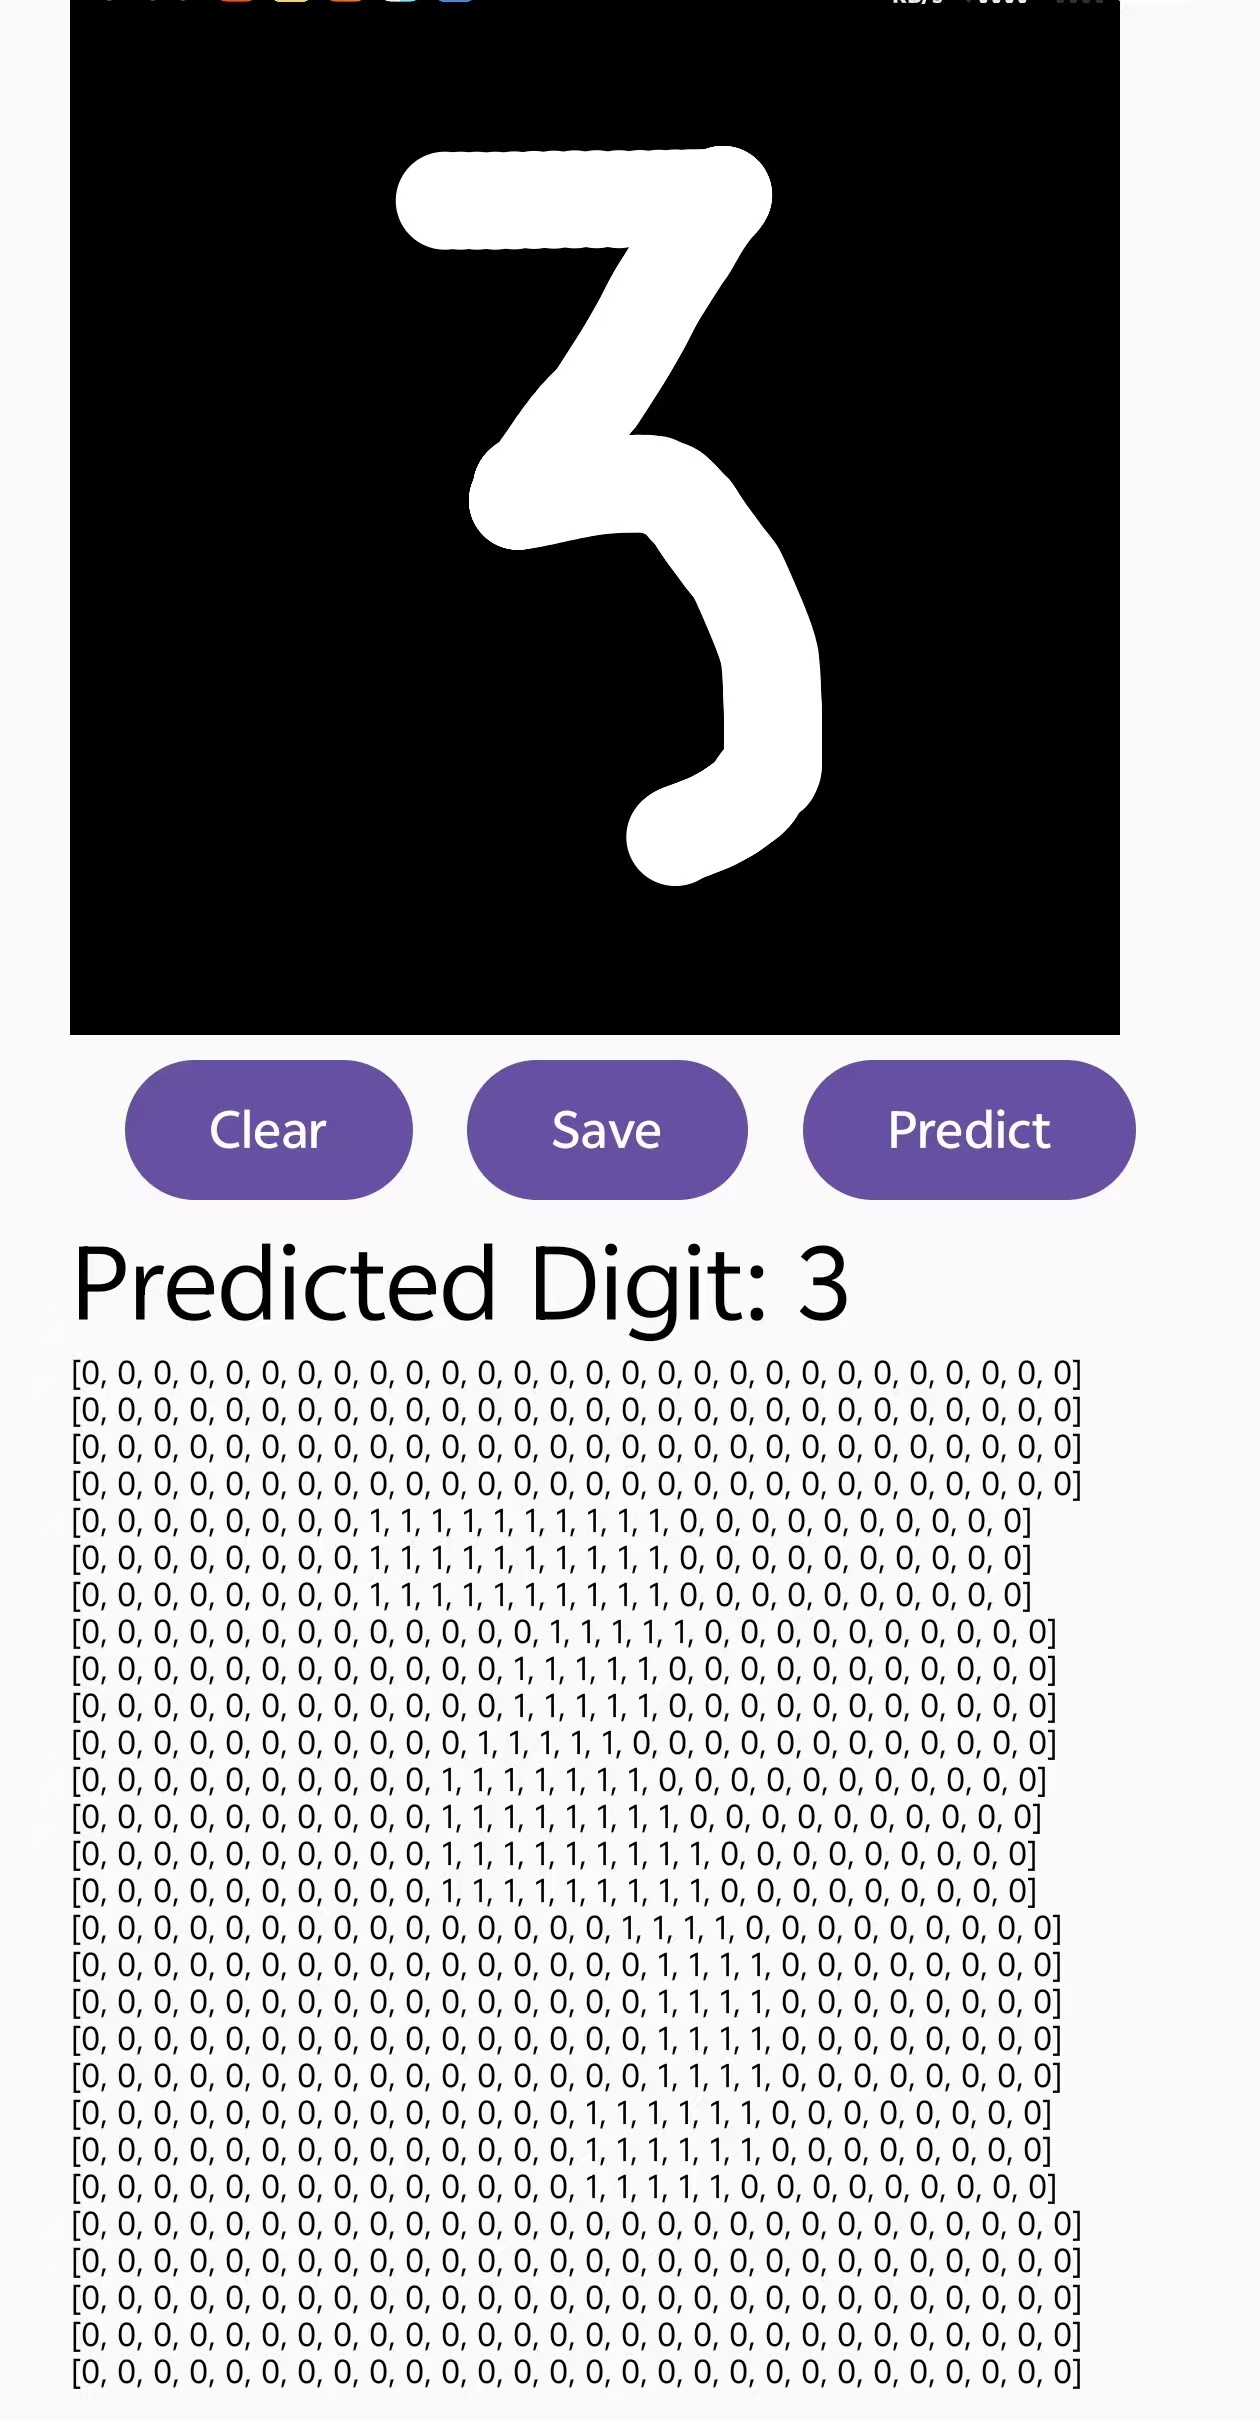
\includegraphics[width=\linewidth]{ASF1}
    \end{minipage}
    \hfill
    \begin{minipage}{0.32\textwidth}
        \centering
        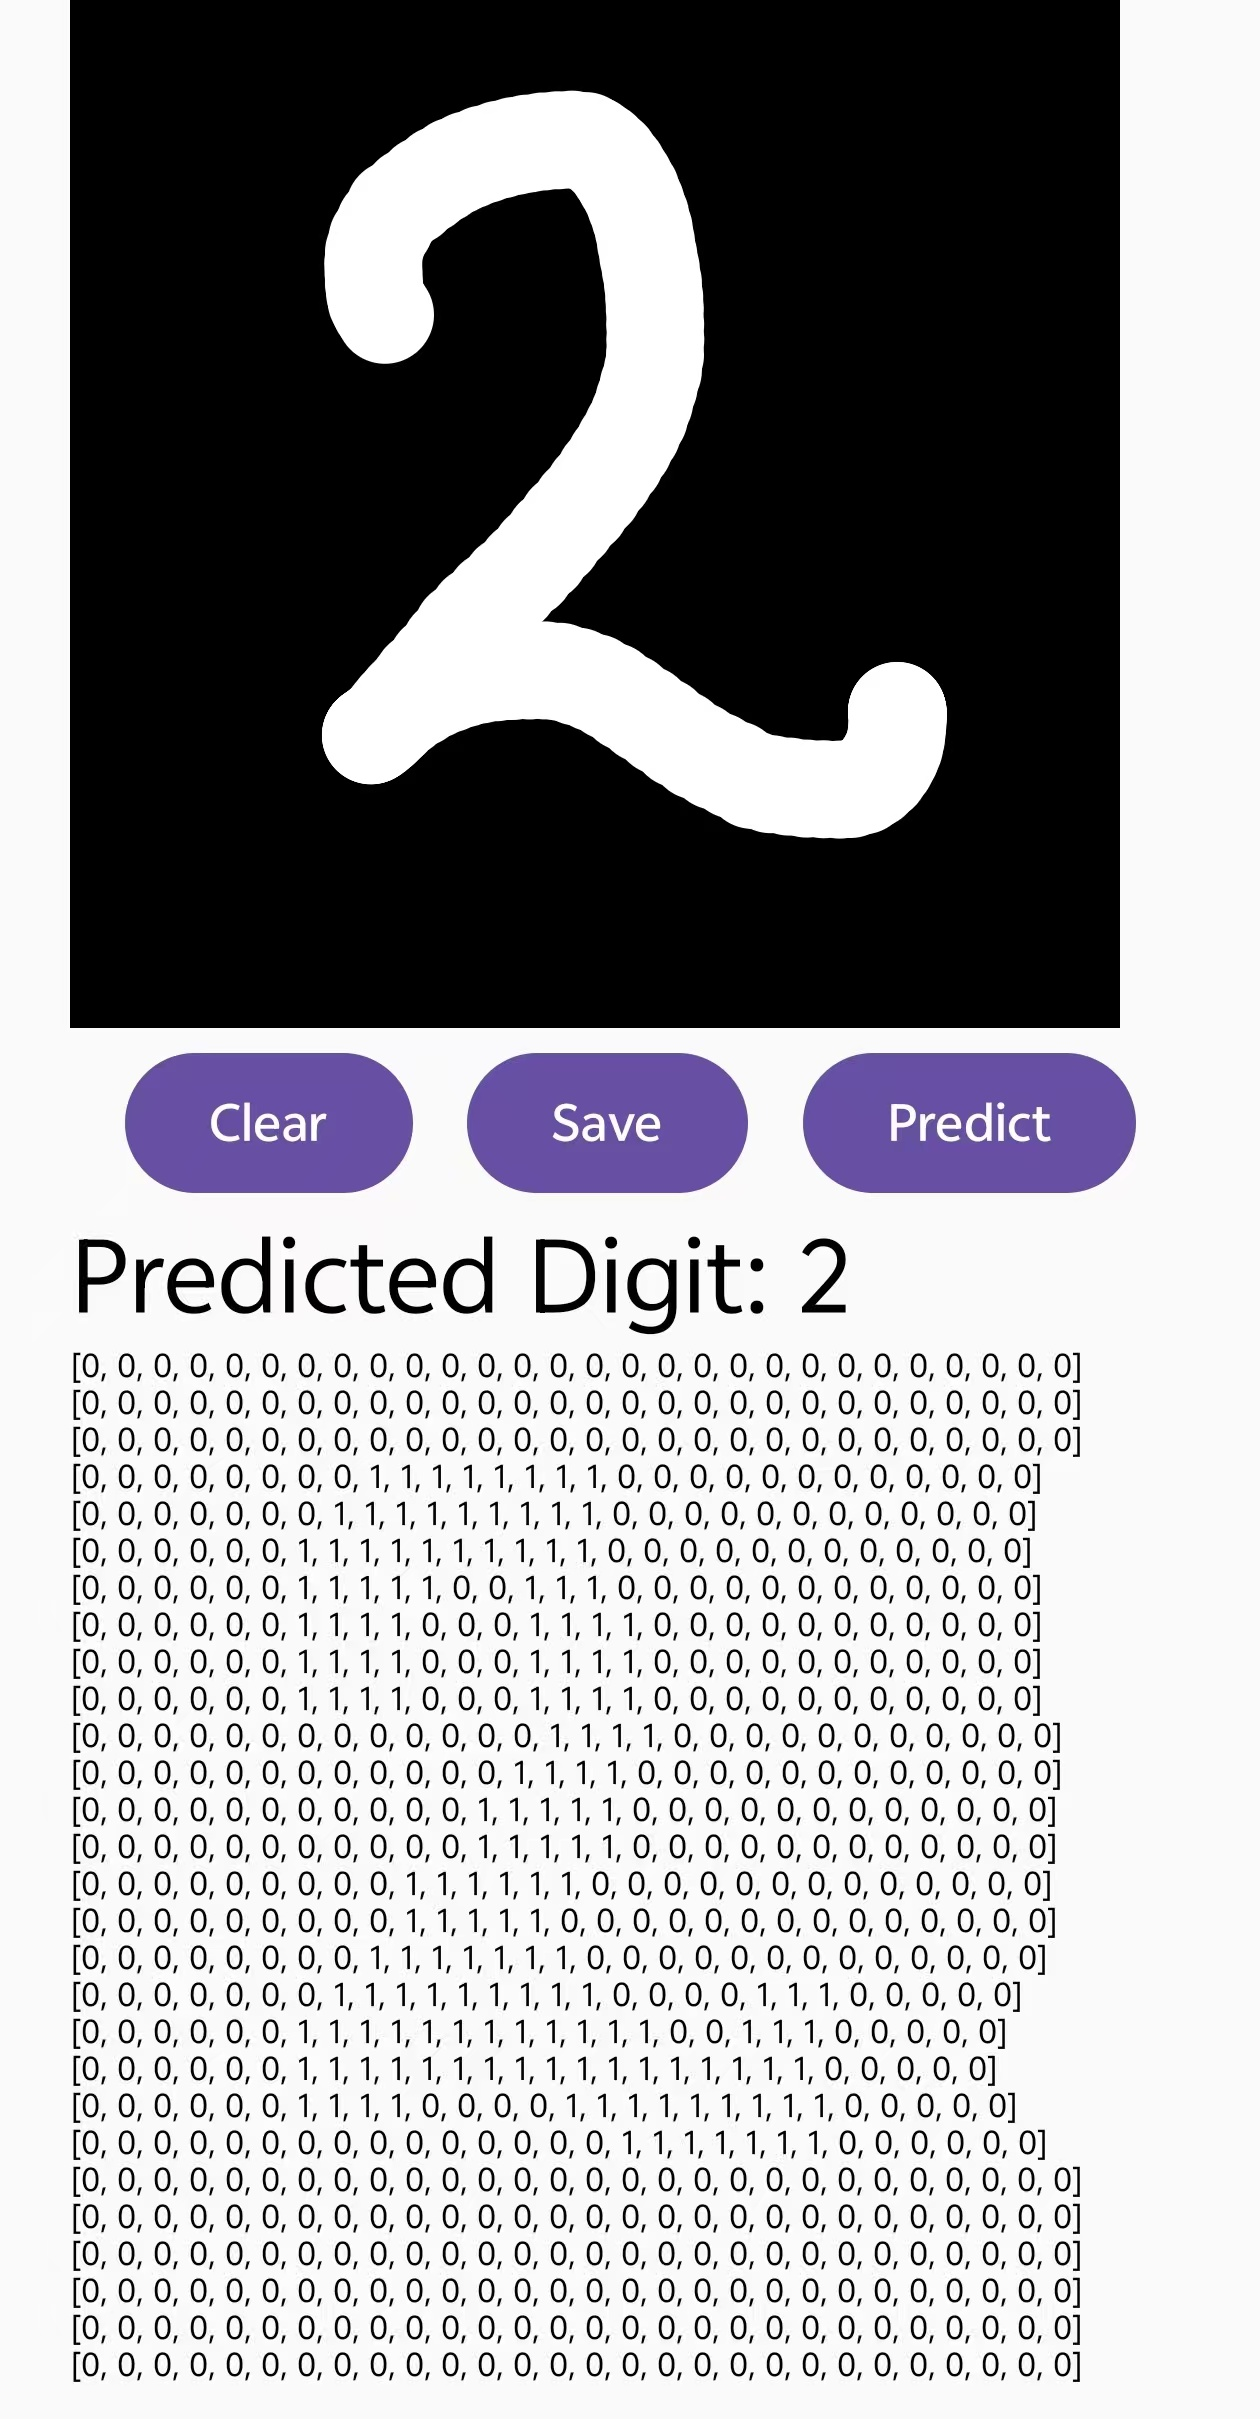
\includegraphics[width=\linewidth]{ASF2}
    \end{minipage}
    \hfill
    \begin{minipage}{0.32\textwidth}
        \centering
        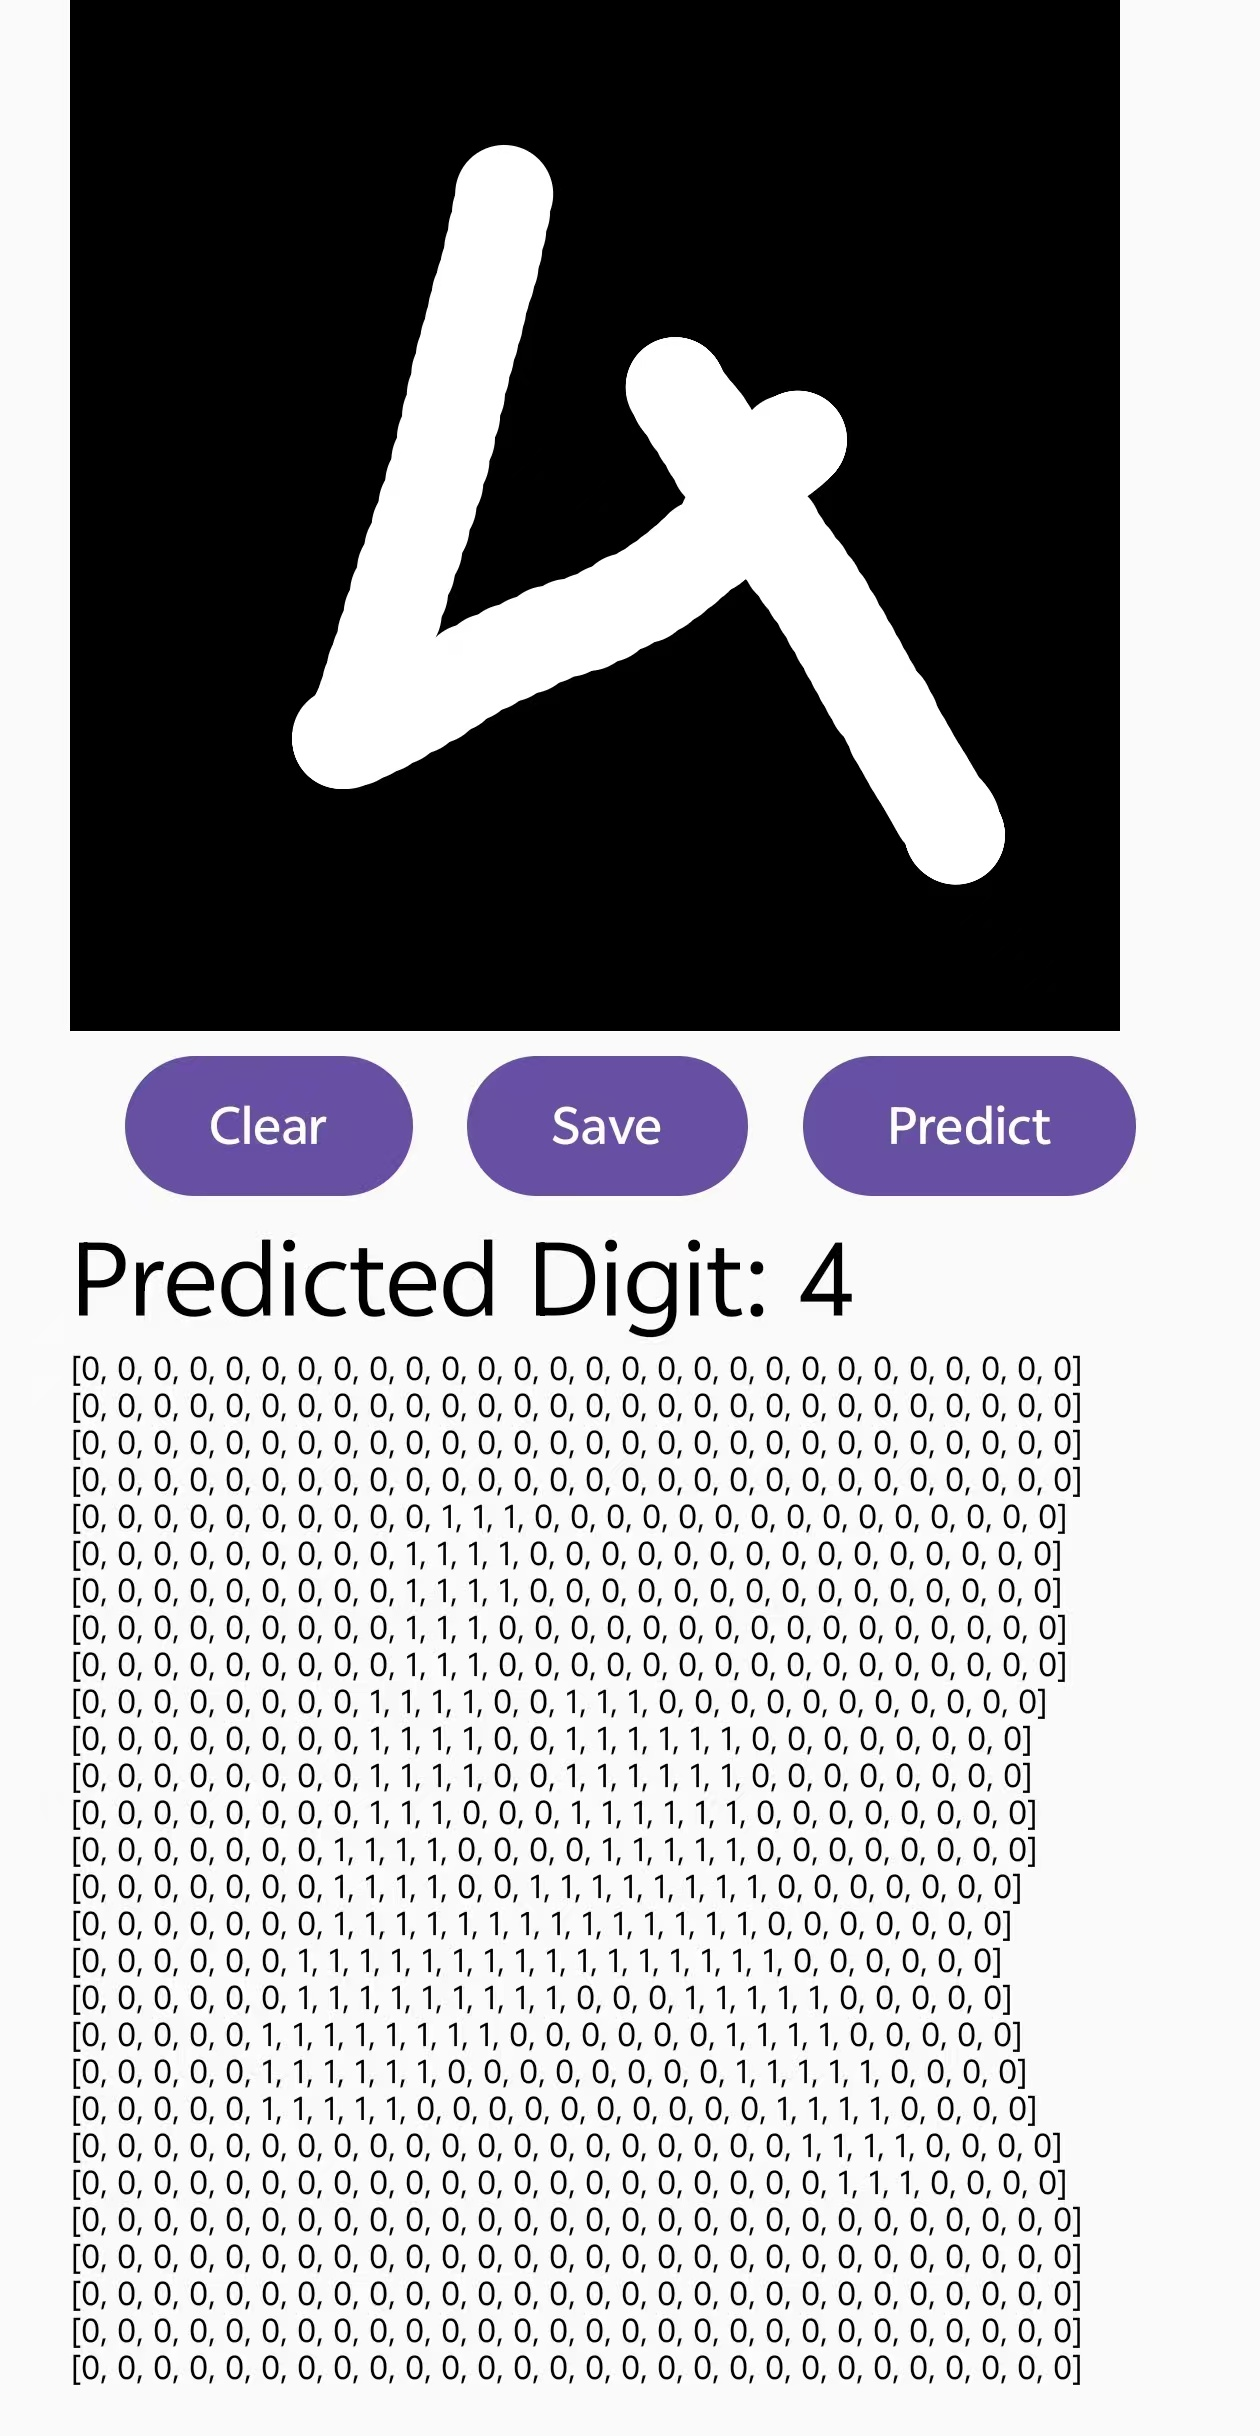
\includegraphics[width=\linewidth]{ASF3}
    \end{minipage}
    \caption{Test results of the digit recognition application on a mobile screen.}
    \label{fig1}
\end{figure}


\section{2D-RNN}\label{2D-RNN}
Image patches are defined as $X_{ij}\in\mathbb{R}^{p\times p}$ for spatial indices $i,j=1,\dots,m$. Each patch is projected into an $f\times f$ low-dimensional feature subspace using shared bilateral projection weights and rectified linear activation:
\[
P_{ij}=\operatorname{ReLU}\big(W^{\text{Feat},L}_{f\times p} X_{ij} W^{\text{Feat},R}_{p\times f} + B^{\text{Feat}}_{f\times f}\big).
\]

We define the network predictive mapping as
\[
D=\mathrm{NN}(H^{t}) = P\big(X \,\big|\, \{H^{s}\mid s<t\}\big) \in [0,1]^{10},
\]
where the $n$-th entry encodes the conditional probability that the input sample $X$ corresponds to digit class $n-1$. The matrix $H^{t}\in\mathbb{R}^{h_1\times h_2}$ denotes the spatial hidden state at grid position $(i,j)$, which is recursively updated through a two-dimensional recurrent transformation:
\begin{equation}
H^{t}=\Phi\big(H^{t-1}, P_{ij}\big),
\end{equation}
with zero boundary initialization conditions
\[
H^{0} = \boldsymbol{0}_{h_1\times h_2}.
\]
We consider a shallow 2D-RNN  for the hidden state by
\begin{equation}
H^{t}=\sigma\left(W^{\text{HP},L}_{h_1\times f} P_{ij} W^{\text{HP},R}_{f\times h_2}
+ W^{\text{H},L}_{h_1\times h_1} H^{t-1} W^{\text{H},R}_{h_2\times h_2}
+ B^{\text{H}}_{h_1\times h_2}\right).
\end{equation}
For inference purposes, the terminal hidden state evaluated at spatial coordinate $(i=m,j=m),$  $t=m^2$ is fed into a dedicated projection layer. Final digit predictions are acquired by computing $\operatorname{argmax}$ over Softmax-normalized output scores with index calibration:
\[
D= \operatorname{ArgMax}\left(\operatorname{Softmax}\big(W^{\text{Inf},L}_{10\times h} H^{m+m-1} W^{\text{Inf},R}_{h\times 1} + B^{\text{Inf}}\big)\right).
\]
In this expression, the $k$-th component of the probability vector $\boldsymbol{d}=[d_1,\dots,d_{10}]$ corresponds to the predicted likelihood for digit class $k-1$, while $\boldsymbol{y}_k$ denotes the matching one-hot encoded ground-truth label.

A customized margin-aware categorical loss function \eqref{CusCatLoss} is constructed for MNIST digit classification tasks.

\section{Experiments and Comparative Analysis: Dense Two-Dimensional Model versus Recurrent Architecture}\label{Experiments and Comparative Analysis}
This section evaluates the predictive performance and computational efficiency of the proposed recurrent neural network framework. We systematically investigate the influence of key hyperparameters, including feature dimension $f$, patch count $m$, individual patch spatial size $p$, and the dimensionality configured for hidden state variables $H$.


\subsection{Feature Dimension $f$}
\begin{example}
We consider a network configuration with $m=4$ (patch size $p=7$), a first hidden layer width $h_1=10$, and a second hidden layer width $h_2=1$, where $h_2$ acts analogously to a category dimension. Table \ref{Tab:5} summarizes the training loss and classification accuracy metrics obtained across a range of feature dimension values $f$. Consistent with our theoretical expectation, expanding the number of network neurons generally improves both training and test accuracy.

When benchmarked against shallow baseline branch networks (presented in Tables \ref{tab:1} and \ref{tab:2}), the proposed architecture yields inferior predictive accuracy under an identical parameter budget. This performance gap is likely attributed to the large volume of small input patches ($m^2=16$) paired with insufficient neuron capacity within the hidden layers, which limits the model's ability to learn discriminative representations for complex input scenarios. In the subsequent example, we increase the number of hidden-layer parameters to enrich the representational capacity of the recursive module, so as to empirically verify this hypothesis.
\end{example}

\begin{table}[htbp]
\centering
\caption{Model performance metrics under varying feature dimension $f$. Training hyperparameters are fixed: batch size = 1000, total training batches = 60, maximum training epochs = 100.}\label{Tab:5}
\label{tab:training_parameters_performance}
\begin{tabular}{cccccc}
\toprule
$f$ &  Num. Neuron & Loss    & Train acc & Test acc & $T$ (s) \\
\midrule
2      & 276  & 0.1820 & 81.4833 & 81.7600 & 13.4645  \\
4      & 338  & 0.1238 & 87.9250 & 88.3700 & 17.7559  \\
6      & 408  & 0.1165 & 88.5183 & 89.5300 & 22.0660  \\
8      & 486  & 0.1227 & 88.1583 & 88.3200 & 26.3529  \\
10     & 572  & 0.0949 & 90.6133 & 90.4300 & 30.6840  \\
12     & 666  & 0.0984 & 90.2850 & 91.0300 & 34.9724  \\
14     & 768  & 0.0987 & 90.3250 & 90.5200 & 39.2767  \\
16     & 878  & 0.0959 & 90.5200 & 90.5700 & 43.5584  \\
18     & 996  & 0.1504 & 85.1000 & 85.0400 & 47.9114  \\
20     & 1122 & 0.0829 & 91.8667 & 92.0800 & 52.2000  \\
\bottomrule
\end{tabular}
\end{table}

%%%%%%%%%%%%%%
\subsection{Hidden State Variables $H$}
\begin{example}
In this experiment, the feature dimension is fixed to $f=20$ with patch configuration $m=4$ ($p=7$). The hidden state dimensions are configured as square matrices satisfying $h_1=h_2$. The network performance under different symmetric hidden state settings is summarized in Table \ref{Tab:6}. Consistent with general neural network behavior, increasing the number of trainable parameters yields progressive performance improvements. 

The optimal configuration achieves a test accuracy of $94.90\%$ utilizing $1500$ neurons. For comparison, the shallow baseline network in Table \ref{tab:2} achieves approximately $96\%$ accuracy under a comparable parameter scale, demonstrating marginal performance differences between the proposed recursive architecture and conventional shallow structures.

\begin{table}[htbp]
\centering
\caption{Model performance with symmetric hidden state dimensions $h_1=h_2$. All experiments adopt fixed training settings: batch size = 1000, 60 training batches, and a maximum of 100 training epochs.}
\label{Tab:6}
\begin{tabular}{cccccc}
\toprule
$h_1=h_2$ &  Num. Neuron & Loss    & Train acc & Test acc & $T$ (s) \\
\midrule
1  & 744  & 0.4970 & 39.1500 & 40.1900 & 52.8897 \\
2  & 804  & 0.3288 & 64.7283 & 65.2700 & 62.0112 \\ 
3  & 870  & 0.1664 & 83.6500 & 82.9700 & 63.4765 \\
4  & 942  & 0.1420 & 86.0917 & 87.5000 & 62.8640 \\
5  & 1020 & 0.0856 & 91.5983 & 92.3200 & 65.9355 \\ 
6  & 1104 & 0.0726 & 92.9117 & 93.4800 & 68.0687 \\
7  & 1194 & 0.0801 & 92.3683 & 92.2100 & 72.4604 \\
8  & 1290 & 0.0657 & 93.6250 & 93.5600 & 68.6180 \\
9  & 1392 & 0.0634 & 93.9117 & 92.1000 & 72.0882 \\
10 & 1500 & 0.0508 & 95.1350 & 94.9000 & 74.4565 \\
\bottomrule
\end{tabular}
\end{table}
\end{example}
%%%%%%%%%%%%%%%%%%%
%\begin{table}[htbp]
%\centering
%\caption{Training parameters and performance. $p=14$, $m=2$, $h_1=h_2=80$, batch size = 500 (120 batches), learning rate = 0.0005, 100 epochs.}
%\label{tab:training_parameters_performance_f80}
%\begin{tabular}{cccccc}
%\toprule
%$f$ & Num. Neuron & Loss    & Train acc & Test acc & $T$ (s) \\
%\midrule
%80      & 41530  & 0.0030 & 99.74 &97.98 & 125.08 \\
%\bottomrule
%\end{tabular}%
%\end{table}



%%%%%%%%%%%%
\subsection{Patch Count and Individual Patch Spatial Dimension $p$}
\begin{example}
This experiment investigates how patch hyperparameters affect model predictive performance and computational overhead. Raising the total number of patches shrinks the spatial context captured within each individual patch, fragmenting global structural information across the input field and turning the image classification task into a harder optimization problem for the recurrent neural network. On the contrary, overly large patch sizes compel the network to integrate irrelevant background pixels when generating prediction outputs.

When the patch size is set to $p=28$, we get $m=1$, and the proposed bilinear formulation degenerates into a conventional dense feedforward neural network. The hidden state update rule
\begin{equation}
H^{1}=\sigma\left(W^{\text{HP},L}_{h_1\times f} P_{ij} W^{\text{HP},R}_{f\times h_2}
+ B^{\text{H}}_{h_1\times h_2}\right)
\end{equation}
collapses to a single dense layer with no recurrent iterative computations. We test a set of alternative patch sizes $p\in\{14,7,4\}$, which correspond to total patch counts $m^2 \in \{4,16,49\}$, respectively. To guarantee fair comparisons across all patch configurations, we fix the feature dimension to $f=40$ and impose symmetric hidden state dimensions $h_1=h_2=40$. Quantitative evaluation metrics for all tested patch sizes are compiled in Table \ref{Tab:7}.

The table demonstrates that smaller patch sizes (and thus more total patches) degrade classification accuracy while drastically extending training runtime, even without reducing the total number of trainable neurons. This observation aligns with a straightforward jigsaw puzzle analogy: reconstructing meaningful labels from numerous tiny patches is far more difficult than reasoning from a small set of large, context-rich patches, just as assembling a jigsaw puzzle with hundreds of tiny fragments poses a greater challenge than completing one with only a few large pieces.

\begin{table}[htbp]
\centering
\caption{Model performance under varying patch spatial dimension $p$. Fixed training hyperparameters: batch size = 500, 120 training batches, maximum 50 training epochs.}
\label{Tab:7}
\begin{tabular}{ccccccc}
\toprule
$p$ & Num. Patches ($m^2$) & Num. Neuron  & Loss & Train Acc. (\%) & Test Acc. (\%) & $T$ (s) \\
\midrule
14 & 4   & 11170  & 0.0158   & 98.48 & 97.98 & 141  \\
7  & 16  & 10610  & 0.0443   & 95.79 & 95.76 & 365 \\
4  & 49  & 10370  & 0.0819   & 92.34 & 90.38 & 970  \\
\bottomrule
\end{tabular}
\end{table}
\end{example}

\subsection{Ablation on Strides}
All preceding patch extraction experiments adopt a fixed uniform stride $s_h = s_v = p$, with identical horizontal and vertical sampling steps enforced for square input matrices, and no boundary pooling or padding applied. We further investigate stride values within the range $s \in \{1,2,\dots,p\}$.

Mathematically, the top-left coordinate $(i,j)$ of each extracted patch follows
\[
i = 1,\,1+s,\,1+2s,\dots,\quad j = 1,\,1+s,\,1+2s,\dots
\]
The stride $s$ controls how many matrix elements the patch window slides across after each extraction. Small $s$ produces an extremely large number of overlapping patches; increasing $s$ gradually reduces the total patch count. When $s=p$, patches are fully non-overlapping; when $s<p$, patches contain overlapping spatial regions.

The sliding window controlled by the stride parameter crops partial regions of the handwritten digit, effectively enriching local feature diversity and thus improving classification accuracy. This mechanism allows the flexible adoption of larger patch windows for feature extraction. In previous settings, only a fixed patch size of 14 was adopted to capture diverse local patterns. By contrast, the proposed framework supports multiple larger patch sizes including 16, 18 and 20, where adaptive stride settings enable stable extraction of complete large-scale patches. As a typical example, the configuration with patch size 16 and stride s=3 yields a total of nine valid feature patches, corresponding to m=3 sampling points along each spatial dimension.

As summarized in Tables \ref{tab:8}, \ref{tab:9} and \ref{tab:10}, we present experimental results across diverse combinations of patch size $p$ and stride $s$, where the model latent dimensions are set to $f=h_1=h_2=20$, $40$, and $80$, respectively. We introduce the generalization gap index, defined as $\text{Train Acc (\%)} - \text{Test Acc (\%)}$; smaller values indicate weaker overfitting and superior generalization performance.

Models in Table \ref{tab:8} contain approximately 3000 trainable parameters and are trained for 100 epochs; all configurations achieve classification accuracy exceeding 97\%. Tables \ref{tab:9} and \ref{tab:10} report models with roughly 11000 and 24000 trainable parameters, respectively. All models adopt a 100-epoch training schedule, and every setup yields around 98\% test classification accuracy.

For Table \ref{tab:8}, the best predictive performance is attained by the configurations $p=16$ and $p=20$ with $m=3$ patches. The minimal generalization gap (weakest overfitting) is observed for $p=12, s=4$.
For Table \ref{tab:9}, the optimal test accuracy is achieved under the $p=13, s=5$ patch setting with $m=4$ patches, which also yields the smallest generalization gap among all configurations in this table.
For Table \ref{tab:10}, the top test performance is observed for the $p=16, s=6$ configuration with $m=3$ patches, while the minimal generalization gap is obtained with $p=13, s=5$.


   \begin{table}[htbp]
  \centering
  \caption{Model performance under different patch size $p$ and stride $s$ with latent dimension $f=h_1=h_2=20$. Training hyperparameters: batch size = 1000, learning rate = 0.0001, total training epochs = 100. The Gap column equals training accuracy minus test accuracy; smaller Gap values represent weaker overfitting. The row with the minimal Gap is marked in bold.}
  \label{tab:8}
  \begin{tabular}{ccccccccc}
    \toprule
    $p$ & $s$ & $m$ & Param. & Train Loss & Train Acc (\%) & Test Acc (\%) & Gap & Time/Epoch (s) \\
    \midrule
20 & 4 & 3 & 3430 & 0.019 & 98.27 & 97.39 & 0.88 & 86.55 \\
14 & 7 & 3 & 3190 & 0.018 & 98.30 & 97.10 & 1.20 & 79.54 \\
13 & 5 & 4 & 3150 & 0.023 & 97.81 & 97.37 & 0.44 & 120.53 \\
16 & 6 & 3 & 3270 & 0.019 & 98.22 & 97.34 & 0.88 & 76.91 \\
\textbf{12} & \textbf{4} & \textbf{5} & \textbf{3110} & \textbf{0.019} & \textbf{98.25} & \textbf{97.81} & \textbf{0.44} & \textbf{175.13} \\
    \bottomrule
  \end{tabular}
\end{table}

\begin{table}[htbp]
  \centering
  \caption{Model performance under different patch size $p$ and stride $s$ with $f=h_1=h_2=40$. Training hyperparameters: batch size = 1000, learning rate = 0.0001, total training epochs = 100. The Gap column is calculated as training accuracy minus test accuracy; smaller Gap values represent weaker overfitting. The row with the minimal Gap is marked in bold.}
  \label{tab:9}
  \begin{tabular}{ccccccccc}
    \toprule
    $p$ & $s$ & $m$ & Param. & Train Loss & Train Acc (\%) & Test Acc (\%) & Gap & Time/Epoch (s) \\ 
    \midrule
20 & 4 & 3 & 11650 & 0.009 & 99.25 & 97.29 & 1.96 & 197.10 \\
14 & 7 & 3 & 11170 & 0.008 & 99.32 & 97.84 & 1.48 & 193.38 \\
\textbf{13} & \textbf{5} & \textbf{4} & \textbf{11090} & \textbf{0.007} & \textbf{99.39} & \textbf{98.33} & \textbf{1.06} & \textbf{323.20} \\
16 & 6 & 3 & 11330 & 0.007 & 99.42 & 98.10 & 1.32 & 198.89 \\
12 & 4 & 5 & 11010 & 0.011 & 99.06 & 97.73 & 1.33 & 476.62 \\
    \bottomrule
  \end{tabular}
\end{table}

\begin{table}[htbp]
  \centering
  \caption{Model performance under different patch size $p$ and stride $s$ with $f=h_1=h_2=80$. Training hyperparameters: batch size = 1000, learning rate = 0.0001, total training epochs = 100. The Gap column is calculated as training accuracy minus test accuracy; smaller Gap values represent weaker overfitting. The row with the minimal Gap is marked in bold.}
  \label{tab:10}
  \begin{tabular}{ccccccccc}
    \toprule
    $p$ & $s$ & $m$ & Param. & Train Loss & Train Acc (\%) & Test Acc (\%) & Gap & Time/Epoch (s) \\ 
    \midrule
20 & 4 & 3 & 24670 & 0.004 & 99.66 & 97.95 & 1.71 & 251.56 \\
14 & 7 & 3 & 23950 & 0.005 & 99.63 & 97.93 & 1.70 & 255.27 \\
13 & 5 & 4 & 23830 & 0.005 & 99.54 & 97.97 & 1.57 & 430.14 \\
16 & 6 & 3 & 24190 & 0.004 & 99.63 & 98.03 & 1.60 & 258.29 \\
\textbf{12} & \textbf{4} & \textbf{5} & \textbf{23710} & \textbf{0.006} & \textbf{99.45} & \textbf{97.93} & \textbf{1.52} & \textbf{706.44} \\
    \bottomrule
  \end{tabular}
\end{table}

We also observe that increasing the number of trainable parameters boosts both training and test accuracy while enlarging the generalization gap, which implies intensified overfitting; additionally, the optimal performance in Tables \ref{tab:9} and \ref{tab:10} occurs at p=13, revealing that neither extremely small nor extremely large patch sizes are ideal, and moderate patch dimensions achieve better classification results.

%%%%%%%%%%%%%%%%%%

% New content added to TwoD_NN.tex on 2026-08-03.
% This file is a standalone copy for review -- the actual content lives inside
% TwoD_NN.tex (MatNet subsection after Table 3; Fashion-MNIST section before
% the Conclusion) and is NOT \input from here. Edit TwoD_NN.tex directly if
% you want changes to make it into the compiled paper.

% ============================================================
% 1) New subsection, inserted after Table 3 (Ultra-Light),
%    before "\subsection{Implementation on Mobile Devices}"
% ============================================================

\subsection{Comparison with Matrix Neural Networks (MatNet)}
As a further point of comparison, we reimplemented the Matrix Neural Network (MatNet) architecture of Gao et al. \cite{Gao2017MatNet} directly from its governing equations (sigmoid hidden layers $X^{(l+1)}=\sigma\big(U^{(l)}X^{(l)}(V^{(l)})^\top+B^{(l)}\big)$, followed by a flattened linear-softmax head), and trained it on MNIST under our own protocol (Adam optimizer, batch size 1000, 100 epochs) to obtain a matched-budget baseline alongside Tables \ref{tab:2} and \ref{tab:3}. Gao et al. report a 5,536-parameter baseline reaching 97.3\% test accuracy and a best 316,160-parameter variant reaching 98.48\%; our reproduction's exact parameter counts differ slightly, since some layer-wiring details are not fully recoverable from the original text alone, and is summarized in Table \ref{tab:matnet}.

\begin{table}[htbp]
\centering
\caption{MatNet \cite{Gao2017MatNet} baseline reproduced under our own training protocol (Adam optimizer, batch size 1000, 100 epochs) on MNIST.}
\label{tab:matnet}
\begin{tabular}{cccccc}
\toprule
Hidden dims & Param. & Train acc (\%) & Test acc (\%) & $T$ (s) \\
\midrule
$20\times16$   & 4986   & 98.08  & 97.44 & 5.76 \\
$40\times32$   & 17674  & 99.39  & 98.05 & 9.63 \\
$80\times64$   & 66186  & 100.00 & 98.34 & 17.93 \\
$160\times160$ & 367370 & 100.00 & 98.38 & 41.61 \\
\bottomrule
\end{tabular}
\end{table}

At comparable parameter counts, the proposed 2D-NN-2L performs on par with MatNet: at $\approx$5K parameters, $\mu_2=47$ (Table \ref{tab:2}) reaches 97.15\% against MatNet's 97.44\% at 4986 parameters, while at the $\approx$$10^5$-parameter scale, $\mu_2=284$ (Table \ref{tab:3}) reaches 98.35\% against MatNet's 98.34\% at 66186 parameters. This indicates that the simpler two-layer, non-flattened bilateral design matches a dedicated matrix-learning baseline despite its substantially lower architectural complexity.


% ============================================================
% 2) New section, inserted before "\section{Conclusion}"
% ============================================================

\section{Generalization to Fashion-MNIST}\label{Fashion-MNIST}
To assess whether the preceding findings extend beyond the comparatively simple MNIST benchmark, we evaluate both the dense 2D-NN-2L (Section~\ref{Experimental Results}) and the 2D-RNN (Section~\ref{2D-RNN}) on Fashion-MNIST \cite{FashionMNIST}, a drop-in replacement dataset of Zalando clothing images sharing MNIST's $28\times28$ grayscale format but posing a substantially harder classification problem. All architectural and training hyperparameters are kept identical to the corresponding MNIST experiments (Adam optimizer, batch size 1000, 100 epochs, Xavier initialization); only the dataset changes.

\subsection{Dense 2D-NN-2L on Fashion-MNIST}

Tables \ref{tab:fashion12}, \ref{tab:fashion13} and \ref{tab:fashion14} repeat the Tiny Ultra-Light sweep of Tables \ref{tab:1}, \ref{tab:2} and \ref{tab:3}, respectively, on Fashion-MNIST, using the same $\mu_2$ values. An adaptive learning rate of the form 
 $$\eta=\frac{\eta_0}{1+ n_e L(n_e)}$$
 (where $n_e$ stands for the epoch iteration, and $\eta_0$ stands for initialrate)
 is used to prevent divergence. 



\begin{table}[htbp]
\centering 
\caption{Shallow 2D-RNN on Fashion-MNIST, same feature-dimension $f$ sweep and training protocol as Table \ref{Tab:1}. With adaptive learning rate per epoch and beginning with initial aggressive rate $\eta=0.1.$}
\label{tab:fashion12}
\begin{tabular}{cccccc}
\toprule
$f$ & Num. Neuron & Loss & Train acc (\%) & Test acc (\%) & $T$ (s) \\
\midrule
1  &  78  & 0.4378 & 46.24 & 46.24 & 0.80    \\
 2  & 148  & 0.2616 & 72.06 & 71.70 & 0.92 \\
 3  & 220  & 0.2269 & 76.64 & 75.96 & 1.32\\
  4  & 294  & 0.2025 & 79.49 & 78.19 & 0.99\\
  5  & 370  & 0.1776 & 82.01 & 80.94 & 1.02\\
  6  & 448  & 0.1633 & 83.18 & 81.71 & 1.08 \\
  7  & 528  & 0.1584 & 83.95 & 82.49 & 1.53\\
  8  & 610  & 0.1438 & 85.31 & 83.99 & 1.08\\
  9  & 694  & 0.1456 & 85.24 & 83.29 & 1.17\\
  10  & 780  & 0.1384 & 86.06 & 84.11 & 1.79\\
  11  & 868  & 0.1330 & 86.61 & 84.52 & 1.72\\
   12  & 958  & 0.1255 & 87.27 & 85.24 & 1.24\\
\bottomrule
\end{tabular}
\end{table}


\begin{table}[htbp]
\centering 
\caption{Dense 2D-NN-2L on Fashion-MNIST, same $\mu_2$ sweep and training protocol as Table \ref{tab:2}.}
\label{tab:fashion13}
\begin{tabular}{cccccc}
\toprule
$\mu_2$ & Num. Neuron & Loss & Train acc (\%) & Test acc (\%) & $T$ (s) \\
\midrule
13  & 1050  & 0.1261 & 87.18 & 85.30 & 1.89\\
17  & 1438  & 0.1141 & 88.63 & 85.87 & 1.57   \\
19  & 1644  & 0.1092 & 89.08 & 85.96 & 2.16 \\
23  & 2080  & 0.1059 & 89.75 & 86.62 & 2.91  \\
31  & 3048  & 0.0932 & 91.09 & 86.83 & 2.9 \\
  41 & 4438  & 0.0822 & 92.39 & 87.69 & 4.68    \\
47  & 5368  & 0.0738 & 93.38 & 88.01 & 10.35\\
53  & 6370  & 0.0754 & 93.08 & 87.56 & 11.43    \\
59  & 7444  & 0.0681 & 93.97 & 87.66 & 8.91 \\
67  & 8988  & 0.0692 & 93.72 & 88.54 & 10.38 \\
71  & 9808  & 0.0639 & 94.30 & 88.37 & 11.65\\ 
\bottomrule
\end{tabular}
\end{table}

\begin{table}[htbp]
\centering
\caption{Training parameters and performance for Ultra-Light 2D-NN-2L on Fashion-MNIST.
Batch size = 1000, 60 batches. Trained with 350 epochs.}
\label{tab:fashion14}
\begin{tabular}{|c|c|c|c|c|c|}
\hline
$\nu_2$ & Num. Neuron & Loss    & Train acc & Test acc & $T$ (s) \\
\hline
284 & 99694&  0.041167    & 96.818
& 89.19& 112.4 \\               
\hline
\end{tabular}
\end{table}   


Compared to Table \ref{tab:2} on MNIST (94.58\%--97.53\% test accuracy over the same $\mu_2$ range), Fashion-MNIST test accuracy is consistently 8--13 percentage points lower, confirming the dataset's greater difficulty. Accuracy increases monotonically with parameter count up to $\mu_2=59$ (88.33\%), after which it plateaus and slightly declines at $\mu_2=71$ (88.23\%), suggesting the model is approaching its capacity limit for this dataset at the Tiny Ultra-Light scale.


\subsection{2D-RNN on Fashion-MNIST}

Tables \ref{tab:14}, \ref{tab:15}, and \ref{tab:16} replicate the feature‑dimension sweep presented in Tables \ref{tab:8}, \ref{tab:9}, and \ref{tab:10} on the Fashion‑MNIST dataset, employing the identical network architecture ($m=4$, $p=7$, $f_1=h_1=h_2$).

For Digit‑MNIST, smaller patch sizes and an increased number of patches improve performance, where the optimal results in Tables \ref{tab:8} and \ref{tab:10} correspond to the final column configurations. However, this trend does not hold for Fashion‑MNIST. In contrast, the best‑performing settings for Fashion‑MNIST tend to appear in the initial columns of the corresponding tables. This discrepancy arises from inherent differences in feature‑extraction behaviour. We note that larger structured neural networks leverage diverse features extracted from varying patch sizes and strides to attain optimal generalization performance.


%{\color{green} Babak: I think this part can be removed or moved to above, not here.\\


%As on MNIST (Table \ref{Tab:5}), accuracy generally improves with $f$, though non-monotonically -- $f=18$ dips below $f=16$, mirroring a similar irregularity at $f=18$ in Table \ref{Tab:5}. The best Fashion-MNIST configuration, $f=16$ (83.31\% test accuracy, 878 neurons), trails the best comparably sized dense configuration in Table \ref{tab:fashion_dense} ($\mu_2=17$, 85.33\% at 1438 neurons) by about two points, consistent with the dense-versus-recurrent gap already observed on MNIST (Section~\ref{Experiments and Comparative Analysis}). Under matched parameter budgets, the dense 2D-NN-2L outperforms the 2D-RNN on Fashion-MNIST as well, indicating that the comparative advantage of the simpler bilateral dense architecture generalizes beyond MNIST.
%}
%%%%%%%%%%%%%%%

\begin{table}[htbp]
  \centering
 
  \caption{Model performance on Fashion-MNIST under different patch size $p$ and stride $s$ with latent dimension $f=h_1=h_2=20$. Training hyperparameters: batch size = 1000, learning rate = 0.0001, total training epochs = 100. The Gap column equals training accuracy minus test accuracy; smaller Gap values represent weaker overfitting. The row with the minimal Gap is marked in bold. Best test accuracy is also highlighted in bold.}
  \label{tab:14}
  \begin{tabular}{ccccccccc}
    \toprule
    $p$ & $s$ & $m$ & Param. & Train Loss & Train Acc (\%) & Test Acc (\%) & Gap & Time/Epoch (s) \\
    \midrule
20 & 4 & 3 & 3430 & 0.13 & 86.20 & 84.60 & 1.60 & 91 \\
14 & 7 & 3 & 3190 & 0.11 & \textbf{88.56} & 86.42 & 2.14 & 94 \\
13 & 5 & 4 & 3150 & 0.12 & 88.08 & \textbf{86.64} & \textbf{1.44} & 150 \\
16 & 6 & 3 & 3270 & 0.11 & 88.35 & 86.32 & 2.03 & 95 \\
12 & 4 & 5 & 3110 & 0.12 & 87.82 & 86.11 & 1.71 & 219\\
    \bottomrule
  \end{tabular}
\end{table}

\begin{table}[htbp]
  \centering
  
  \caption{Model performance on Fashion-MNIST under different patch size $p$ and stride $s$ with latent dimension $f=h_1=h_2=40$. Training hyperparameters: batch size = 1000, learning rate = 0.0001, total training epochs = 100. The Gap column equals training accuracy minus test accuracy; smaller Gap values represent weaker overfitting. The row with the minimal Gap is marked in bold. Best test accuracy is also highlighted in bold.}
  \label{tab:15}
  \begin{tabular}{ccccccccc}
    \toprule
    $p$ & $s$ & $m$ & Param. & Train Loss & Train Acc (\%) & Test Acc (\%) & Gap & Time/Epoch (s) \\
    \midrule
 20 & 4 & 3 & 11650 & 0.09 & 91.02 & 87.95 & 3.07 & 135  \\
 14 & 7 & 3 & 11170 & 0.10 & 89.77 & 87.46 & 2.31 & 199\\
 13 & 5 & 4 & 11090 & 0.11 & 89.00 & 87.00 & 2.01 & 249 \\
 16 & 6 & 3 & 11330 & 0.09 & \textbf{91.16} & \textbf{88.55} & 2.61 & 124 \\
 12 & 4 & 5 & 11010 & 0.13 & 86.54 & 85.29 & \textbf{1.25} & 355 \\
    \bottomrule
  \end{tabular}
\end{table}

\begin{table}[htbp]
  \centering

  \caption{Model performance on Fashion-MNIST under different patch size $p$ and stride $s$ with latent dimension $f=h_1=h_2=80$. Training hyperparameters: batch size = 1000, learning rate = 0.0001, total training epochs = 100. The Gap column equals training accuracy minus test accuracy; smaller Gap values represent weaker overfitting. The row with the minimal Gap is marked in bold. Best test accuracy is also highlighted in bold.}
  \label{tab:16}
  \begin{tabular}{ccccccccc}
    \toprule
    $p$ & $s$ & $m$ & Param. & Train Loss & Train Acc (\%) & Test Acc (\%) & Gap & Time/Epoch (s) \\
    \midrule
    20 & 4 & 3 & 42490 & 0.09 & \textbf{90.31} & \textbf{88.28} & 2.03 & 455\\
    14 & 7 & 3 & 41530 & 0.10 & 90.13 & 87.72 & 2.41 & 465 \\
    13 & 5 & 4 & 41370 & 0.10 & 89.73 & 87.63 & 2.10 & 929\\
    16 & 6 & 3 & 41850 & 0.11 & 88.99 & 87.38 & 1.62 & 486\\
    12 & 4 & 5 & 41210 & 0.13 & 86.15 & 84.42 & 1.73 & 227\\
    \bottomrule
  \end{tabular}
\end{table}



%%%%%%%%%%%%%%%%%%%%%%%
\section{Conclusion}\label{Conclusion}
%In this paper, we introduced a novel 2D neural network framework that preserves spatial structure and captures full contextual information for image recognition tasks. The proposed method was validated on the MNIST dataset, achieving fast training and high classification accuracy that is competitive with models without feature extraction or attention modules. The results confirm the effectiveness and efficiency of the proposed 2D network design, supporting its potential for integration with modern lightweight AI techniques toward fast training and low-cost development. Furthermore, the proposed approach enables rapid construction of mobile applications, especially for educational scenarios such as alphabet learning tools for languages that lack dedicated resources.




This paper introduced a unified matrix-learning framework for ultra-lightweight image recognition, comprising a dense two-dimensional neural network (2D-NN) and a two-dimensional recurrent neural network (2D-RNN). The dense model preserves the matrix structure of images through bilateral left–right transformations, avoiding vectorization while capturing full spatial dependencies, with forward and backward propagation derived entirely in matrix form; the recurrent model extends this principle to image patches via recursive hidden-state propagation with shared bilateral projection weights. Within the proposed hierarchy of lightweight scales (super-tiny, tiny, ultra-light), the shallow two-layer dense architecture reached 94.78\% test accuracy on MNIST with fewer than 1K neurons, 97.53\% under 10K, and 98.35\% at the ultra-light scale—surpassing several neuromorphic and optoelectronic baselines and rivaling classical CNN and MLP designs—with CPU training completed in minutes and without feature extraction or attention modules. A real-time Android application confirmed practical deployability on resource-constrained edge devices.

The comparative study exposed clear trade-offs: under identical parameter budgets, the dense 2D-NN attains slightly higher accuracy at substantially lower training cost, while the 2D-RNN offers flexible patch-based spatial context aggregation. Enlarging feature and hidden-state dimensions improves accuracy but widens the generalization gap; moderate patch sizes are preferable, since excessive fragmentation degrades both accuracy and training speed; and overlapping patch extraction with adaptive strides enriches local feature diversity, driving the 2D-RNN to approximately 98\% test accuracy with only about 24K parameters while simultaneously reducing overfitting.

Two additional experiments situate these results more broadly. First, a from-equations reproduction of the Matrix Neural Network (MatNet) baseline \cite{Gao2017MatNet} shows the proposed 2D-NN-2L performing on par at matched parameter counts (e.g. 98.35\% vs. 98.34\% at the $\approx10^5$-parameter scale), despite its simpler two-layer, non-flattened design. Second, evaluating both architectures on Fashion-MNIST -- a harder benchmark sharing MNIST's format -- confirms that the dense model's advantage over the 2D-RNN under matched parameter budgets generalizes beyond MNIST, with the dense model reaching 88.33\% and the 2D-RNN 83.31\% test accuracy in the Tiny Ultra-Light regime.

Future work will pursue deeper 2D architectures, lightweight attention and feature-extraction modules, data augmentation, extensions to color images and larger benchmarks, and the incorporation of fractional-order memory dynamics into the recurrent formulation. The fast training and minimal resource demands of the proposed networks further favor rapid mobile application development, particularly educational tools such as handwriting and alphabet learning for languages lacking dedicated resources.





\section*{Data Availability}
The dataset used in this study is publicly available at \url{http://yann.lecun.com/exdb/mnist/.} 
All trained model weights, Code, and supporting data are deposited in Zenodo at \url{https://doi.org/10.5281/zenodo.20169149} and \url{https://github.com/ZahraAlijani/FRNN}.


\section*{Conflict of Interest Declaration}
The authors declare that there are no conflicts of interest regarding the publication of this paper. There is no financial or non-financial relationship with any organization or individual that could influence the results and conclusions presented in this study.


\section*{Funding}

The described research originates from the project Research of Excellence on Digital Technologies and Wellbeing CZ.02.01.01/00/22\_008/0004583 which is co-financed by the European Union.
The article has been produced with the financial support of the European Union under the REFRESH – Research Excellence For REgion Sustainability and High-tech Industries project number CZ.10.03.01/00/22\_003/0000048 via the Operational Programme Just Transition.

\begin{thebibliography}{99}

\bibitem{xavier_glorot}
Glorot, X.; Bengio, Y. Understanding the difficulty of training deep feedforward neural networks.
In \textit{Proceedings of the 13th International Conference on Artificial Intelligence and Statistics (AISTATS)},
Sardinia, Italy, 2010, pp.~249--256.

\bibitem{he_init}
He, K.; Zhang, X.; Ren, S.; Sun, J. Delving deep into rectifiers: Surpassing human-level performance on ImageNet classification.
In \textit{Proceedings of the IEEE International Conference on Computer Vision (ICCV)}, 2015, pp.~1026--1034.

\bibitem{kingma2014adam}
Kingma, D.P.; Ba, J. Adam: A method for stochastic optimization.
arXiv preprint arXiv:1412.6980, 2014.

\bibitem{Cortes1995}
Cortes, C.; Vapnik, V. Support-vector networks.
\textit{Mach. Learn.} \textbf{1995}, \textbf{20}, 273--297.

\bibitem{Rumelhart1986}
Rumelhart, D.E.; Hinton, G.E.; Williams, R.J. Learning representations by back-propagating errors.
\textit{Nature} \textbf{1986}, \textbf{323}, 533--536.

\bibitem{LeCun1998}
LeCun, Y.; Bottou, L.; Bengio, Y.; Haffner, P. Gradient-based learning applied to document recognition.
\textit{Proc. IEEE} \textbf{1998}, \textbf{86}(11), 2278--2324.

\bibitem{Krizhevsky2012}
Krizhevsky, A.; Sutskever, I.; Hinton, G.E. ImageNet classification with deep convolutional neural networks.
In \textit{Advances in Neural Information Processing Systems (NIPS)}, 2012, pp.~1097--1105.

\bibitem{Zhu2022}
Zhu, C.; Liu, H.; Wang, W.; et al. Optical synaptic devices with ultra-low power consumption for neuromorphic computing.
\textit{Light Sci. Appl.} \textbf{2022}, \textbf{11}, 337.

\bibitem{Beyeler2013}
Beyeler, M.; Dutt, N.D.; Krichmar, J.L. Categorization and decision-making in a neurobiologically plausible spiking network using a STDP-like learning rule.
\textit{Neural Networks} \textbf{2013}, \textbf{48}, 109--124.

\bibitem{Song2024}
Song, A.; Kottapalli, S.N.M.; Goyal, R.; et al. Low-power scalable multilayer optoelectronic neural networks enabled with incoherent light.
\textit{Nat. Commun.} \textbf{2024}, \textbf{15}, 10692.

\bibitem{Hopfield1982} Hopfield, J.J. Neural networks and physical systems with emergent collective computational abilities. \textit{Proc. Natl. Acad. Sci. USA} \textbf{1982}, \textbf{79}(8), 2554--2558. 

\bibitem{Jordan1986} Jordan, M.I. Serial order: A parallel distributed processing approach. Technical Report ICS-8604, Institute for Cognitive Science, University of California, San Diego, 1986.

\bibitem{Elman1990} Elman, J.L. Finding structure in time. \textit{Cogn. Sci.} \textbf{1990}, \textbf{14}(2), 179--211.

\bibitem{Werbos1990} Werbos, P.J. Backpropagation through time: What it does and how to do it. \textit{Proc. IEEE} \textbf{1990}, \textbf{78}(10), 1550--1560. 

\bibitem{Bengio1994} Bengio, Y.; Simard, P.; Frasconi, P. Learning long-term dependencies with gradient descent is difficult. \textit{IEEE Trans. Neural Netw.} \textbf{1994}, \textbf{5}(2), 157--166. 

\bibitem{Hochreiter1997} Hochreiter, S.; Schmidhuber, J. Long short-term memory. \textit{Neural Comput.} \textbf{1997}, \textbf{9}(8), 1735--1780. 

\bibitem{Schuster1997} Schuster, M.; Paliwal, K.K. Bidirectional recurrent neural networks. \textit{IEEE Trans. Signal Process.} \textbf{1997}, \textbf{45}(11), 2673--2681. 

\bibitem{Gers2000} Gers, F.A.; Schmidhuber, J.; Cummins, F. Learning to forget: Continual prediction with LSTM. \textit{Neural Comput.} \textbf{2000}, \textbf{12}(10), 2451--2471. 

\bibitem{Graves2006} Graves, A.; Fernandez, S.; Gomez, F.; Schmidhuber, J. Connectionist temporal classification: Labelling unsegmented sequence data with recurrent neural networks. In \textit{Proceedings of the 23rd International Conference on Machine Learning (ICML)}, 2006, pp.~369--376. 

\bibitem{Mikolov2010} Mikolov, T.; Karafiát, M.; Burget, L.; Černocký, J.; Khudanpur, S. Recurrent neural network based language model. In \textit{Proceedings of Interspeech}, 2010, pp.~1045--1048.

\bibitem{Pascanu2013} Pascanu, R.; Mikolov, T.; Bengio, Y. On the difficulty of training recurrent neural networks. In \textit{Proceedings of the 30th International Conference on Machine Learning (ICML)}, 2013, pp.~1310--1318. 

\bibitem{Cho2014GRU} Cho, K.; van Merriënboer, B.; Gülçehre, Ç.; Bahdanau, D.; Bougares, F.; Schwenk, H.; Bengio, Y. Learning phrase representations using RNN encoder-decoder for statistical machine translation. arXiv preprint arXiv:1406.1078, 2014. 

\bibitem{Sutskever2014} Sutskever, I.; Vinyals, O.; Le, Q.V. Sequence to sequence learning with neural networks. In \textit{Advances in Neural Information Processing Systems (NeurIPS)}, 2014, pp.~3104--3112. 

\bibitem{Bahdanau2014} Bahdanau, D.; Cho, K.; Bengio, Y. Neural machine translation by jointly learning to align and translate. arXiv preprint arXiv:1409.0473, 2014.

\bibitem{Vaswani2017} Vaswani, A.; Shazeer, N.; Parmar, N.; Uszkoreit, J.; Jones, L.; Gomez, A.N.; Kaiser, Ł.; Polosukhin, I. Attention is all you need. In \textit{Advances in Neural Information Processing Systems (NeurIPS)}, 2017, pp.~5998--6008. 

\bibitem{Feng2024} Feng, L.; Tung, F.; Ahmed, M.O.; Bengio, Y.; Hajimirsadeghi, H. Were RNNs all we needed? arXiv preprint arXiv:2410.01201, 2024.
\bibitem{Han2015} Han, S.; Pool, J.; Tran, J.; Dally, W. Learning both weights and connections for efficient neural networks. \textit{Advances in Neural Information Processing Systems (NeurIPS)} \textbf{2015}, 1135--1143. 
\bibitem{Howard2017} Howard, A.G.; Zhu, M.; Chen, B.; et al. MobileNets: Efficient convolutional neural networks for mobile vision applications. arXiv preprint arXiv:1704.04861, 2017.
\bibitem{Sandler2018} Sandler, M.; Howard, A.; Zhu, M.; Zhmoginov, A.; Chen, L.C. MobileNetV2: Inverted residuals and linear bottlenecks. \textit{Proc. IEEE/CVF Conference on Computer Vision and Pattern Recognition} \textbf{2018}, 4510--4520. \bibitem{Tan2019} Tan, M.; Le, Q. EfficientNet: Rethinking model scaling for convolutional neural networks. \textit{Proc. International Conference on Machine Learning (ICML)} \textbf{2019}, 6105--6114. 
\bibitem{Kolda2009} Kolda, T.G.; Bader, B.W. Tensor decompositions and applications. \textit{SIAM Review} \textbf{2009}, \textbf{51}(3), 455--500. 
\bibitem{Novikov2015} Novikov, A.; Podoprikhin, D.; Osokin, A.; Vetrov, D. Tensorizing neural networks. \textit{Advances in Neural Information Processing Systems (NeurIPS)} \textbf{2015}, 442--450. 
\bibitem{Gao2017MatNet} Gao, J.; Guo, Y.; Wang, Z. Matrix Neural Networks.
In \textit{Advances in Neural Networks -- ISNN 2017}, Lecture Notes in
Computer Science, vol. \textbf{10261}; Springer: Cham, \textbf{2017};
pp. 313--320.
\bibitem{Renanse2023} Renanse, A.; Sharma, A.; Chandra, R. Memory capacity of recurrent neural networks with matrix representation. \textit{Neurocomputing} \textbf{2023}, \textbf{560}, 126824.
\bibitem{Graves2007MDRNN} Graves, A.; Fern\'{a}ndez, S.; Schmidhuber, J. Multi-dimensional recurrent neural networks. In \textit{Artificial Neural Networks -- ICANN 2007}, Lecture Notes in Computer Science, vol.~\textbf{4668}; Springer: Berlin, Heidelberg, \textbf{2007}; pp.~549--558.
\bibitem{Byeon2014} Byeon, W.; Liwicki, M.; Breuel, T.M. Texture classification using 2D LSTM networks. In \textit{Proceedings of the 22nd International Conference on Pattern Recognition (ICPR)}, \textbf{2014}; pp.~1144--1149.
\bibitem{Shiri2026FRNN} Shiri, B.; Alijani, Z.; Dassios, I.; Baleanu, D. Incommensurate fractional recurrent neural networks. \textit{Neurocomputing} \textbf{2026}, \textbf{669}, 132535. https://doi.org/10.1016/j.neucom.2025.132535.
\bibitem{Shiri2026Math} Shiri, B.; Liu, C.X.; Liu, Y. Generalized incommensurate 
fractional differential systems: Commensurate and incommensurate weight analyses, 
existence-uniqueness, HU stability, and neural network applications. 
\textit{Mathematics} \textbf{2026}, \textbf{14}(8), 1308.
\bibitem{Molek2025PRL} Molek, V.; Alijani, Z. Fractional concepts in neural 
networks: Enhancing activation functions. \textit{Pattern Recognition Letters} \textbf{2025}, \textbf{190}, 126--132.
\bibitem{FashionMNIST} Xiao, H.; Rasul, K.; Vollgraf, R. Fashion-MNIST: a novel image
dataset for benchmarking machine learning algorithms. arXiv preprint arXiv:1708.07747, 2017.






\end{thebibliography}






\end{document}